\documentclass[9pt,pdf,utf8,hyperref={unicode},aspectratio=169]{beamer}

%Привычный шрифт для математических формул
\usefonttheme[onlymath]{serif}
\mode<presentation>
{
    \usetheme{boxes}
    \beamertemplatenavigationsymbolsempty

    \setbeamercovered{transparent}
    \setbeamertemplate{navigation symbols}{}
    
    \setbeamertemplate{footline}[frame number]
    \setbeamertemplate{caption}[numbered]
    % \setbeamersize{text margin left=0.5em, text margin right=0.5em}
}

% Дополнительные библиотеки
\usepackage[T2A]{fontenc}
\usepackage[english, russian]{babel}
\usepackage[utf8]{inputenc}
\usepackage{amsmath,amssymb}
\usepackage{indentfirst}
\usepackage{changepage}
\usepackage{enumerate}
\usepackage{mathtools}
\usepackage{multicol}
\usepackage{multirow}
\usepackage{ragged2e}
\usepackage{multicol}
\usepackage{diagbox}
\usepackage{wrapfig}
\usepackage{comment}
\usepackage{subfig}
\usepackage{array}
\usepackage{color}
\usepackage{tikz}
\usepackage{url}
\usepackage{bm}

\usetikzlibrary{trees}

% Определение дополнительных функций
\DeclareMathOperator*{\plim}{\mathop{plim}}
\DeclareMathOperator{\prob}{\mathbf{P}\!}
\DeclareMathOperator{\arctanh}{arctanh}
\DeclareMathOperator{\mmode}{mode}
\DeclareMathOperator{\rank}{rank}
\DeclareMathOperator{\diag}{diag}
\DeclareMathOperator{\sign}{sign}
\DeclareMathOperator{\cov}{cov}
\DeclareMathOperator{\pow}{pow}
\DeclareMathOperator{\med}{med}

\def\argmin#1{ \mathop{\text{argmin}}\limits_{#1} }
\def\argmax#1{ \mathop{\text{argmax}}\limits_{#1} }

% Основная часть

\title{Прикладной статистический анализ данных\\~\\~\\\large{Проверка параметрических гипотез}}

\author{Андрей Грабовой}
\date{}


\begin{document}
\tikzstyle{every node}=[draw=black,thick,anchor=west]
\tikzstyle{selected}=[draw=red,fill=red!30]
\tikzstyle{optional}=[dashed,fill=gray!50]

\begin{frame}
    \titlepage
\end{frame}


\begin{frame}{Проверка гипотез}
%%%%%%%%%%%%%%%%%%%%%%%%%%%%%%%%%%%%%%%%%%%%%%%%%%%%%%%%%%%%%%%%%%%%%%%
% Проверка гипотез - основной инструмент этого курса, если в итоге вы в нём не разберётесь, считайте, что зря потратили время. Имеется выборка из случайной величины X, которая имеет неизвестное распределение P. Кроме того, выдвинута нулевая гипотеза об этом распределении (например, ”P принадлежит некоторому семейству распределений ?”) и альтернативная гипотеза (например, общая альтернатива ”P не принадлежит ?”). Требуется проверить, глядя на выборку, какая из двух гипотез, нулевая или альтернативная, более вероятна. Для этого используется некоторая статистика T , которая обладает очень важным свойством: если нулевая гипотеза справедлива, то точно известно, какое у статистики распределение, а если справедлива альтернатива, то распределение статистики — какое-то другое. Распределение F (x) называется нулевым распределением статистики, а пара, состоящая из статистики и нулевого распределения, образует статистический критерий для проверки нулевой гипотезы против альтернативы. Мы получаем данные, то есть, реализацию выборки, считаем на них значение статистики и по нему вычисляем так называемый достигаемый уровень значимости, или p-value, представляющий собой вероятность получить такое или ещё более экстремальное значение статистики при справедливости нулевой гипотезы. "Экстремальность" определяется относительно альтернативной гипотезы: допустим, если при альтернативе более вероятными являются большие значения статистики, то именно их мы и будем считать экстремальными. Затем p-value сравнивают с порогом ?, который называется уровнем значимости. Чаще всего ? = 0.05. Если p ? ?, то нулевая гипотеза отвергается в пользу альтернативы. Если p > ?, то нулевая гипотеза не отвергается.
%%%%%%%%%%%%%%%%%%%%%%%%%%%%%%%%%%%%%%%%%%%%%%%%%%%%%%%%%%%%%%%%%%%%%%%
	\only<1>{
		\begin{center}
			\vspace{-10pt}
			\begin{tabular}{rl}
				выборка:                        & $X^n=\left(X_1,\ldots,X_n\right), \; X \sim \prob \in \Omega$         \\
				нулевая гипотеза:               & $H_0\colon \prob\in\omega, \;\; \omega\in\Omega$ \\
				альтернатива:                   & $H_1\colon \prob\notin\omega$ \\
				статистика:                     & $T\left(X^n\right), \;\; T\left(X^n\right)\sim F\left(x\right) \;\text{при}\; \prob\in\omega$ \\
				& \;\;\;\;\;\;\;\;\;\;\;\;\;\; $T\left(X^n\right)\not\sim F\left(x\right) \;\text{при}\; \prob\notin\omega$ \\
				\multicolumn{2}{c}{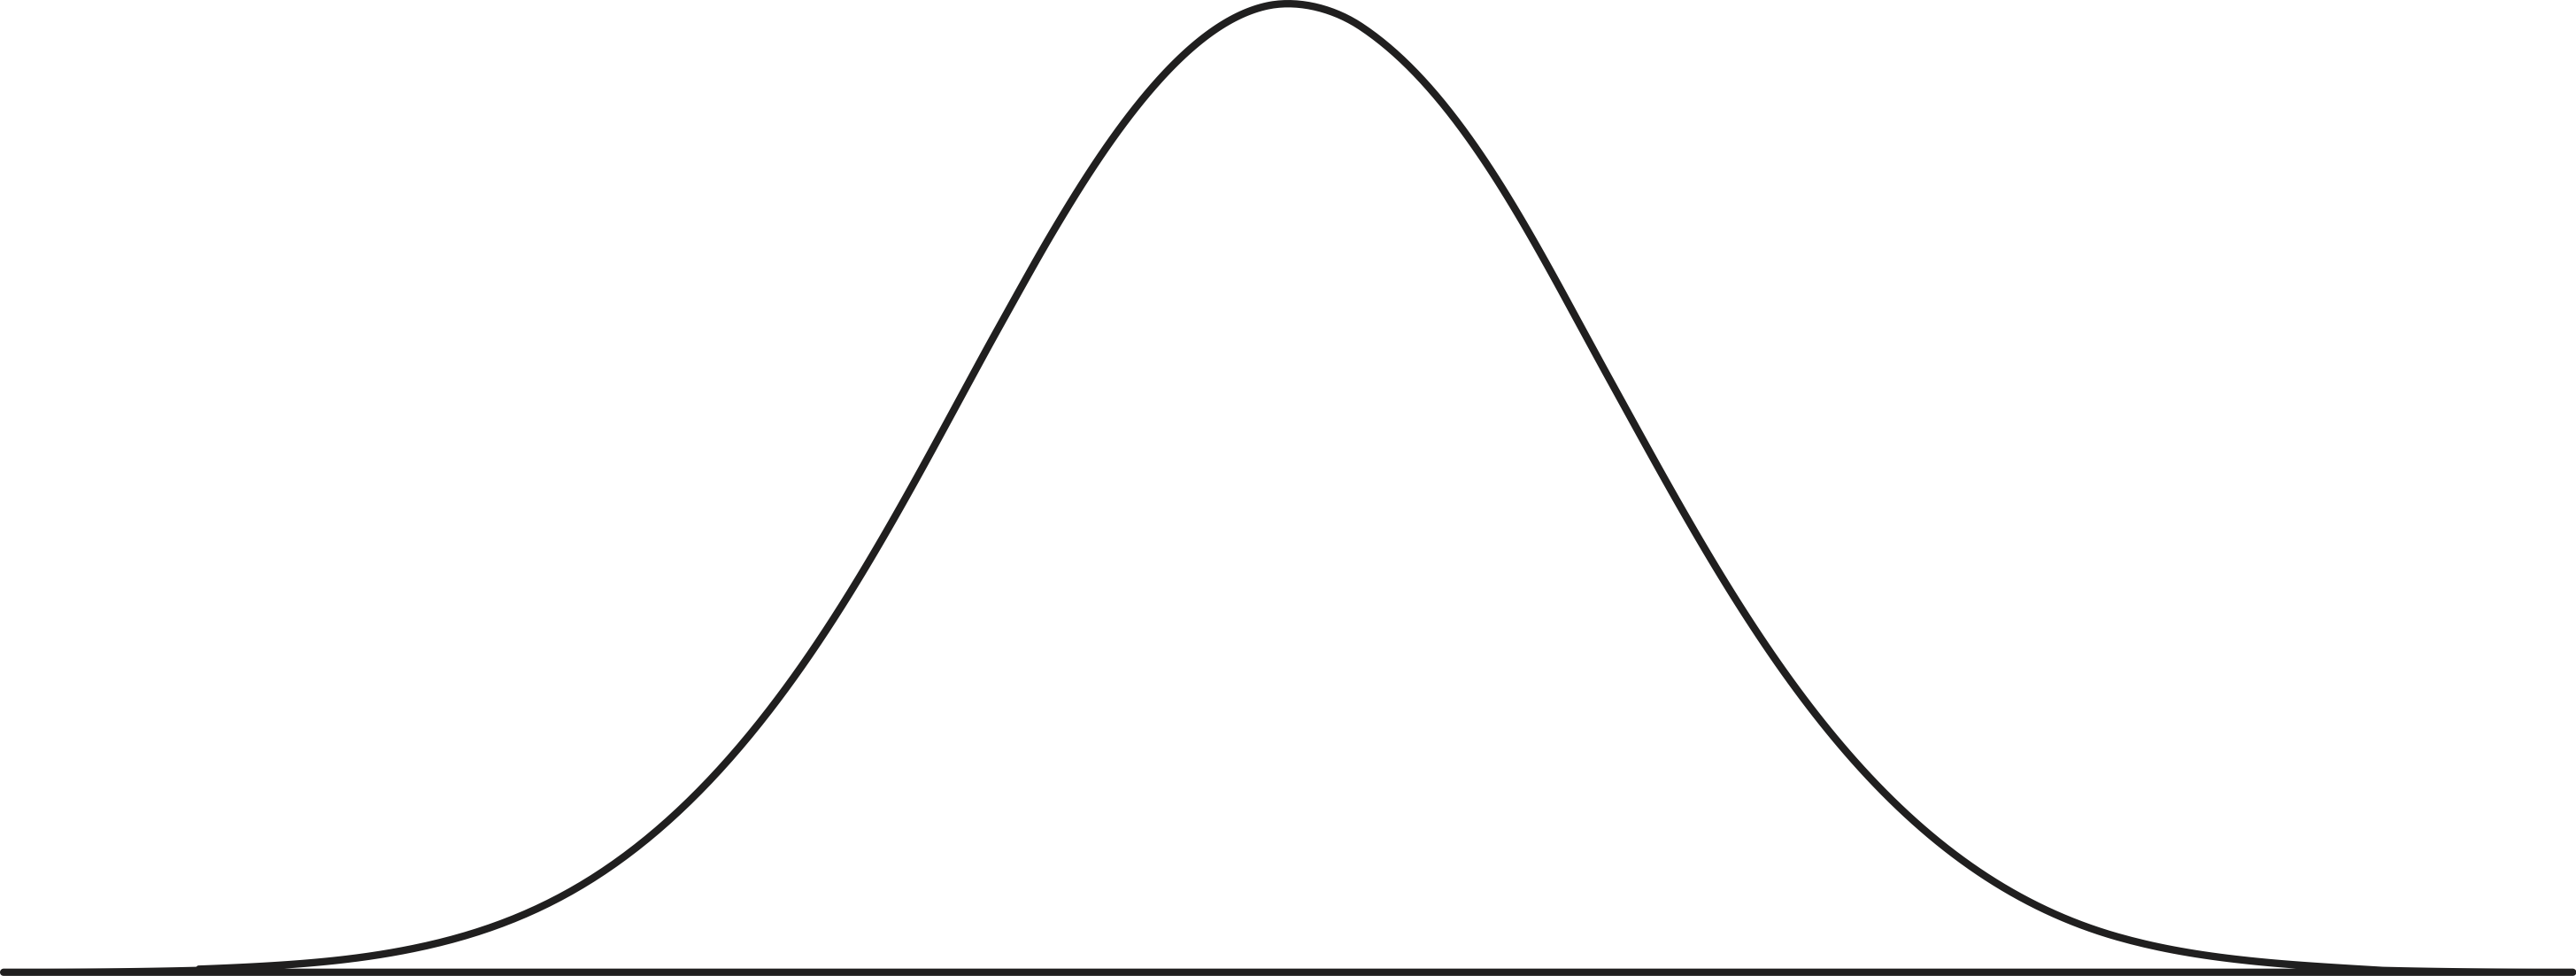
\includegraphics[width=0.35\textwidth]{stats1.png}} \\
				реализация выборки:             & $x^n=\left(x_1,\ldots,x_n\right)$ \\
				реализация статистики:          & $t = T \left(x^n\right)$ \\
				достигаемый уровень значимости: & $p\left(x^n\right)$~--- вероятность при $H_0$ получить \\
				& $T \left(X^n\right)=t$ или ещё более экстремальное\\
				\multicolumn{2}{c}{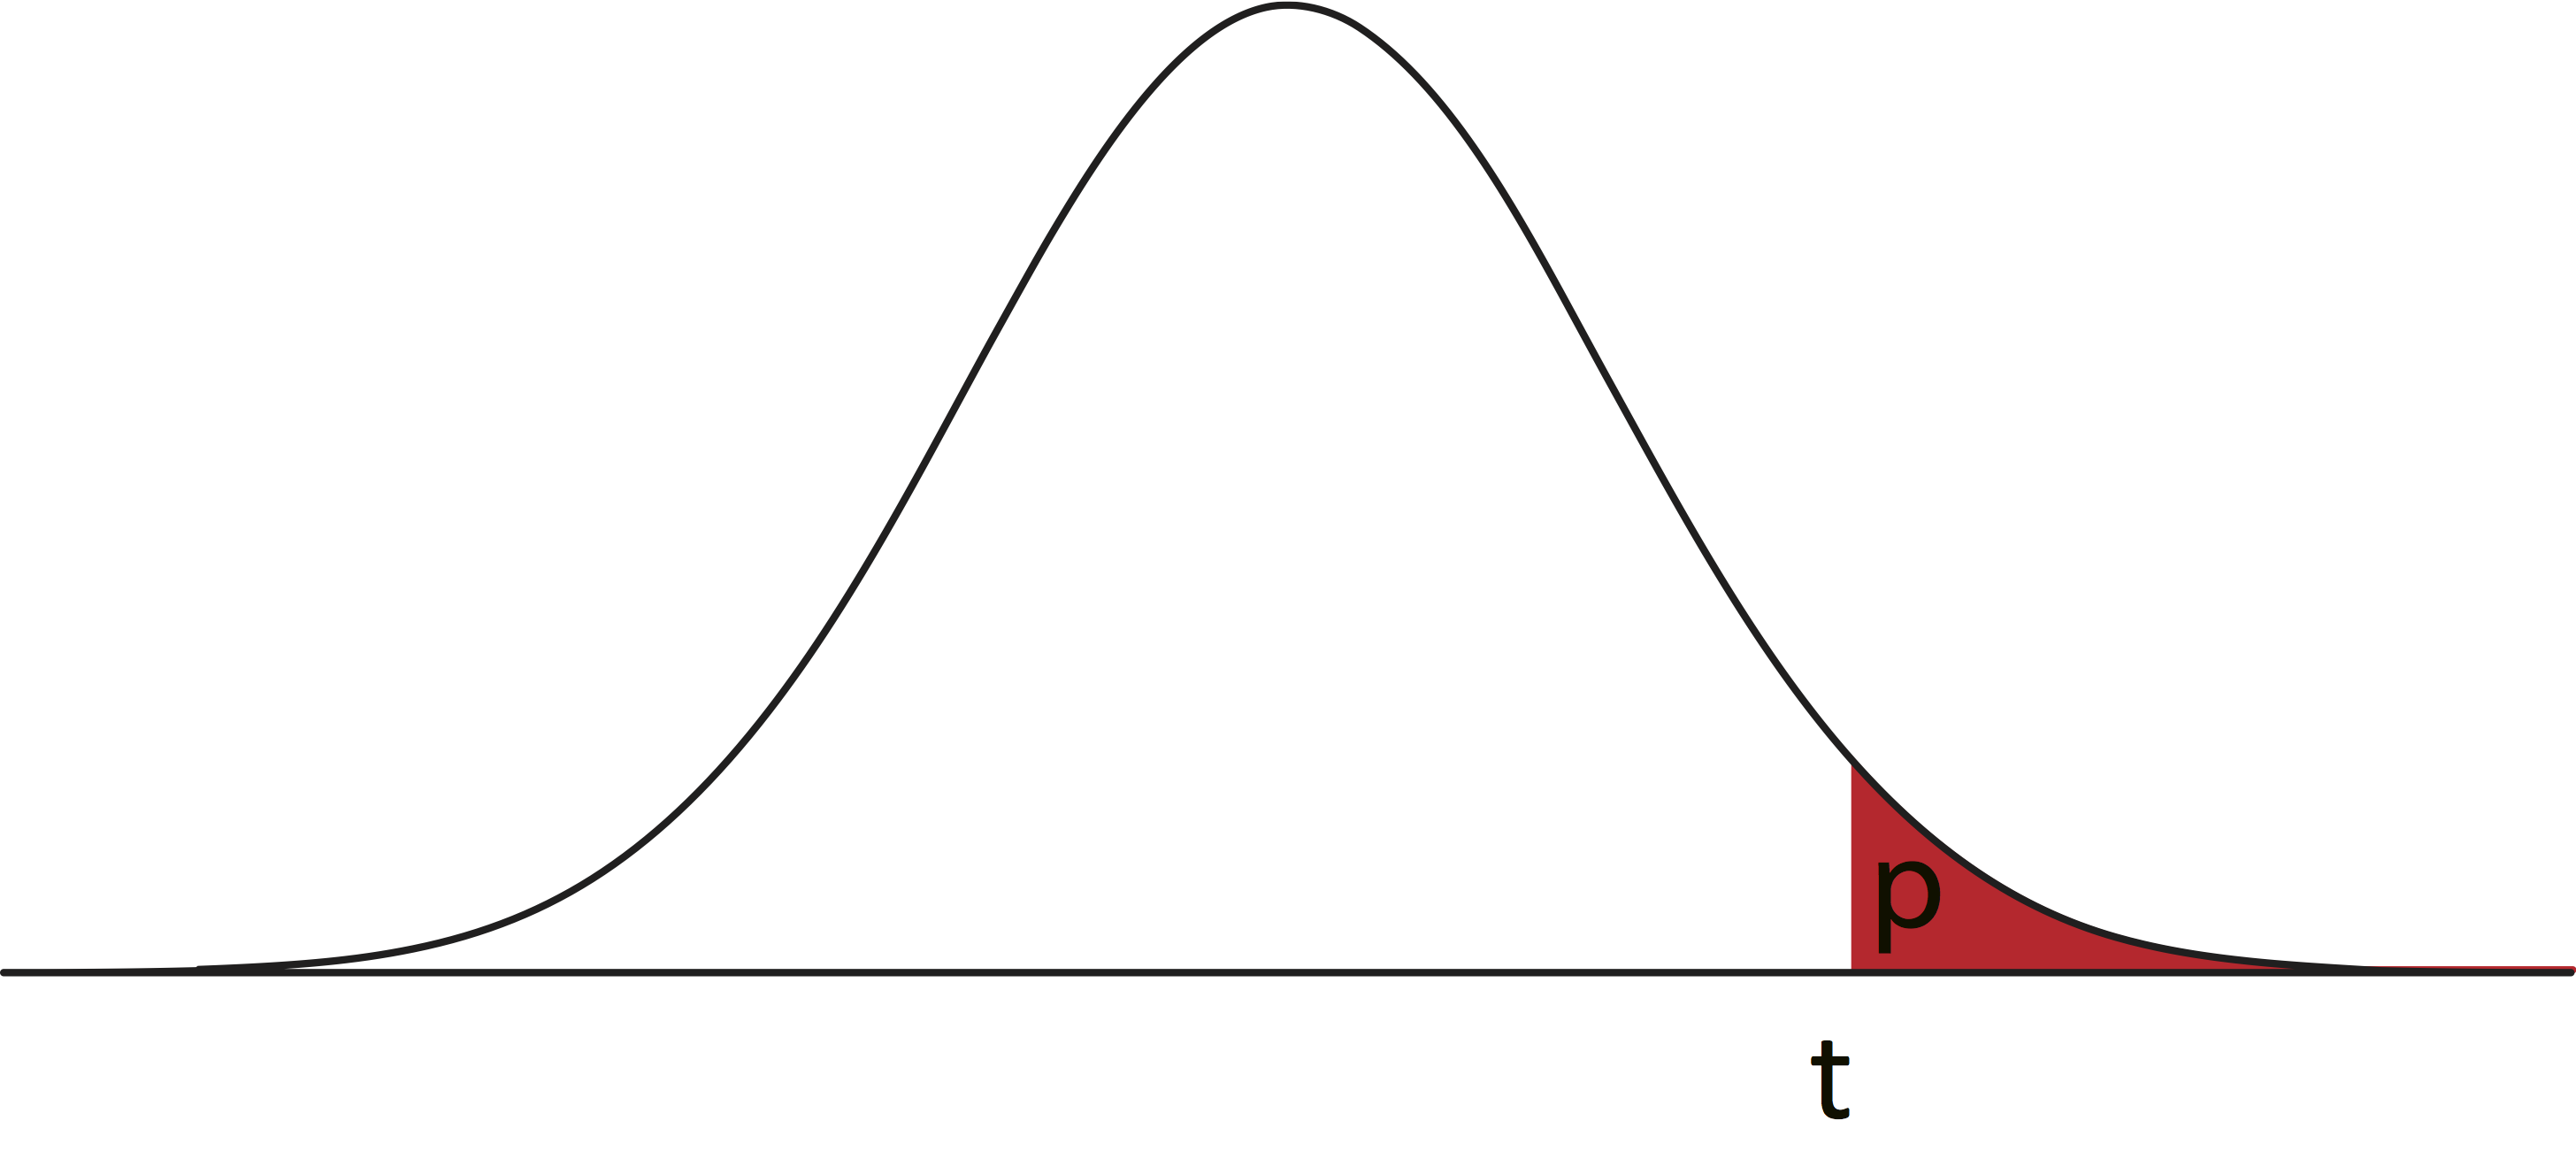
\includegraphics[width=0.35\textwidth]{stats2.png}} \\
				\multicolumn{2}{c}{ $p\left(x^n\right) = \prob\left(T\geq t\left|H_0\right.\right)$ } \\
				\multicolumn{2}{c}{Гипотеза отвергается при $p\left(x^n\right)\leq\alpha,\;\;\alpha$~--- уровень значимости} \\
			\end{tabular}
		\end{center}
	}
	\only<2>{
		\vspace{-3pt}
		\begin{center}
			\includegraphics[height=0.9\textheight]{rememberkids.png}
		\end{center}
	}
\end{frame}

%%%%%%%%%%%%%%%%%%%%%%%%%%%%%%%%%%%%%%%%%%%%%%%%%%%%%%%%%%%%%%%%%%%%%%%
% Это занятие посвящено параметрическим критериям проверки гипотез. Эти критерии называются параметрическими потому, что в проверяемых ими гипотезах высказывается предположение о значении параметра распределений, из которых предположительно взята выборка.
%%%%%%%%%%%%%%%%%%%%%%%%%%%%%%%%%%%%%%%%%%%%%%%%%%%%%%%%%%%%%%%%%%%%%%%

\section{Нормальное распределение}
%%%%%%%%%%%%%%%%%%%%%%%%%%%%%%%%%%%%%%%%%%%%%%%%%%%%%%%%%%%%%%%%%%%%%%%
% Благодаря центральной предельной теореме и удобству вывода критериев для нормально распределённых выборок методы, основанные на предположении о нормальности данных, наиболее широко распространены.
%%%%%%%%%%%%%%%%%%%%%%%%%%%%%%%%%%%%%%%%%%%%%%%%%%%%%%%%%%%%%%%%%%%%%%%

\subsection{Некоторые задачи для нормальных выборок}
\begin{frame}[label=onesample]{Виды задач: одновыборочные}
	\begin{tikzpicture}[%
	grow via three points={one child at (0.5,-0.7) and
		two children at (0.5,-0.7) and (0.5,-1.4)},
	edge from parent path={(\tikzparentnode.south) |- (\tikzchildnode.west)}]
	\node {$X^n \sim N(\mu, \sigma^2)$}	
	child { node {$H_0\colon \mu = \mu_0$}
		child { node {$\sigma$ известна   \hyperlink{ztest1}{\beamerbutton{1}} }}
		child { node {$\sigma$ неизвестна \hyperlink{ttest1}{\beamerbutton{3}} }}
	}			
	child [missing] {}				
	child [missing] {}				
	child { node {$H_0\colon \sigma = \sigma_0$ \hyperlink{chitest1}{\beamerbutton{2}}}};
	\end{tikzpicture}
\end{frame}

\begin{frame}[label=twosample]{Виды задач: двухвыборочные}
	\begin{tikzpicture}[%
	grow via three points={one child at (0.5,-0.7) and
		two children at (0.5,-0.7) and (0.5,-1.4)},
	edge from parent path={(\tikzparentnode.south) |- (\tikzchildnode.west)}]
	\node {$X_1^{n_1} \sim N(\mu_1, \sigma_1^2), \;\; X_2^{n_2} \sim N(\mu_2, \sigma_2^2)$}	
	child { node {$H_0\colon \mu_1 = \mu_2$}
		child { node {$X_1,X_2$ независимые}
			child { node {$\sigma_1, \sigma_2$ известны \hyperlink{ztest2u}{\beamerbutton{4}} }}	
			child { node {$\sigma_1, \sigma_2$ неизвестны \hyperlink{ttest2u}{\beamerbutton{5}} }}
		}
		child [missing] {}				
		child [missing] {}
		child { node {$X_1,X_2$ связанные \hyperlink{ttest2p}{\beamerbutton{6}} }}
	}		
	child [missing] {}				
	child [missing] {}	
	child [missing] {}				
	child [missing] {}	              			
	child { node {$H_0\colon \sigma_1 = \sigma_2$ \hyperlink{ftest}{\beamerbutton{7}}}};
	\end{tikzpicture}
	
\end{frame}
\subsection{Одновыборочные задачи}
\begin{frame}[label=ztest1]{\hyperlink{onesample}{\beamerbutton{1}} Z-критерий}
	\only<1>{
		\begin{center}
			\begin{tabular}{rl}
				выборка:                        & $X^n=\left(X_1,\ldots,X_n\right), X \sim N\left(\mu, \sigma^2\right)$\\
				& $\sigma$ известна         \\
				нулевая гипотеза:               & $H_0\colon \mu=\mu_0$ \\
				альтернатива:                   & $H_1\colon \mu<\neq>\mu_0$ \\
				статистика:                     & $Z\left(X^n\right) = \frac{\bar{X}-\mu_0}{\sigma / \sqrt{n}}$ \\
				нулевое распределение:          & $N(0,1)$\\
			\end{tabular}
			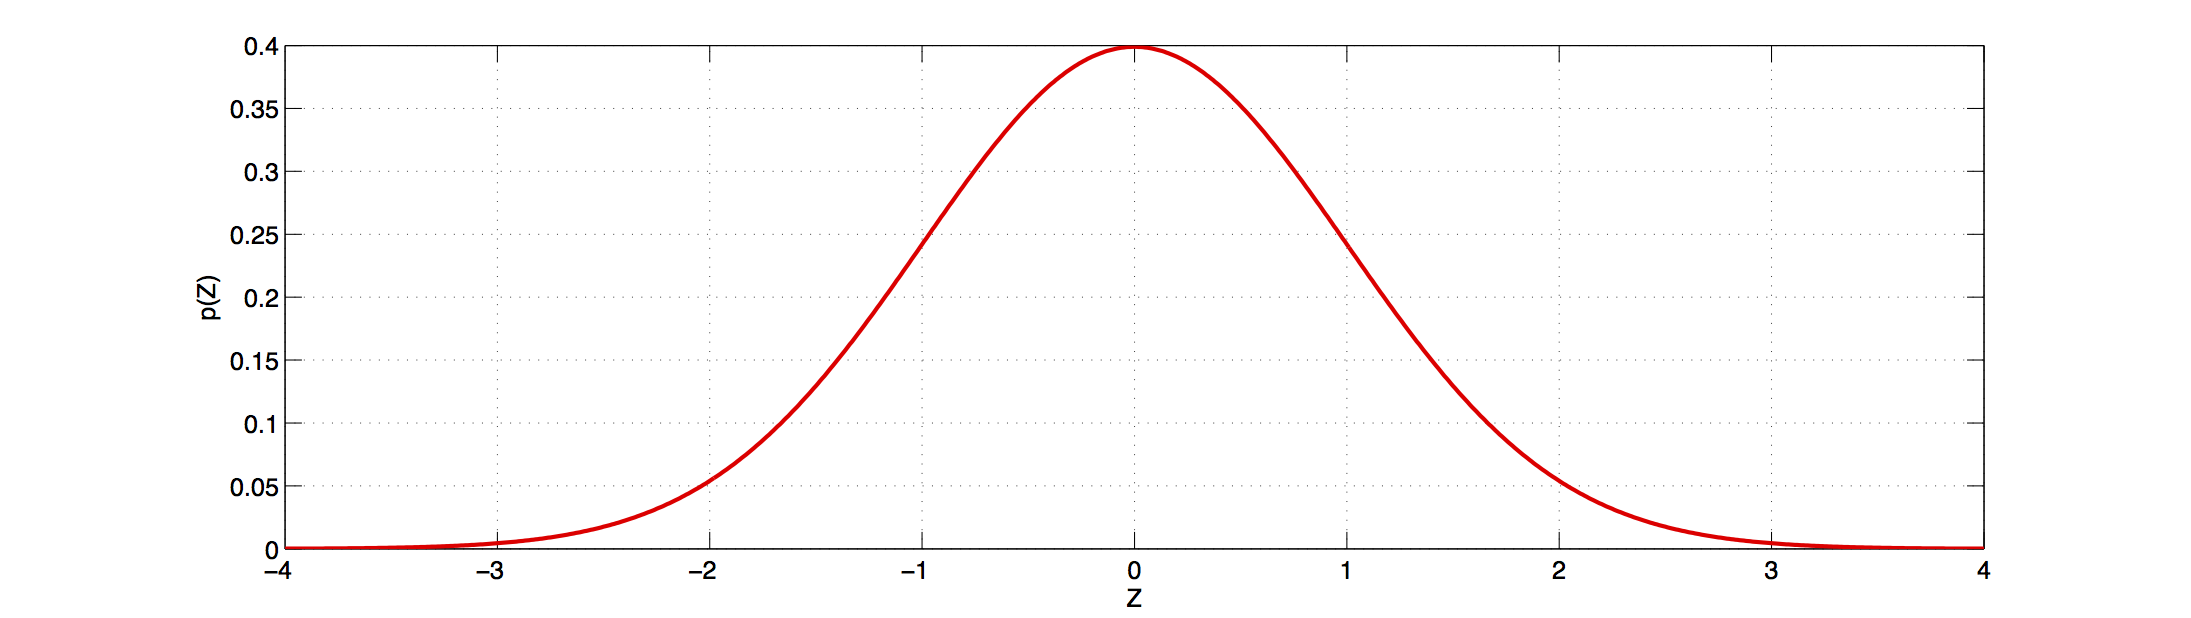
\includegraphics[width=0.7\textwidth]{norm.png}
		\end{center}
	достигаемый уровень значимости:
	$$p\left(Z\right) = \begin{cases}
	1-F_{N(0,1)}(Z), & H_1 \colon \theta>\theta_0, \\
	F_{N(0,1)}(Z), & H_1 \colon \theta<\theta_0, \\
	2\left(1-F_{N(0,1)}(|Z|)\right), & H_1 \colon \theta\neq\theta_0. \\
	\end{cases}
	$$
	}
    
	\only<2>{
		\begin{center}            
			\begin{tabular}{rl}
				выборка:                        & $X^n=\left(X_1,\ldots,X_n\right), X \sim N\left(\mu, \sigma^2\right)$\\
				& $\sigma$ известна         \\
				нулевая гипотеза:               & $H_0\colon \mu=\mu_0$ \\
				альтернатива:                   & $H_1\colon \mu < \mu_0$ \\
				статистика:                     & $Z\left(X^n\right) = \frac{\bar{X}-\mu_0}{\sigma / \sqrt{n}}$ \\
				нулевое распределение:          & $N(0,1)$\\
			\end{tabular}
			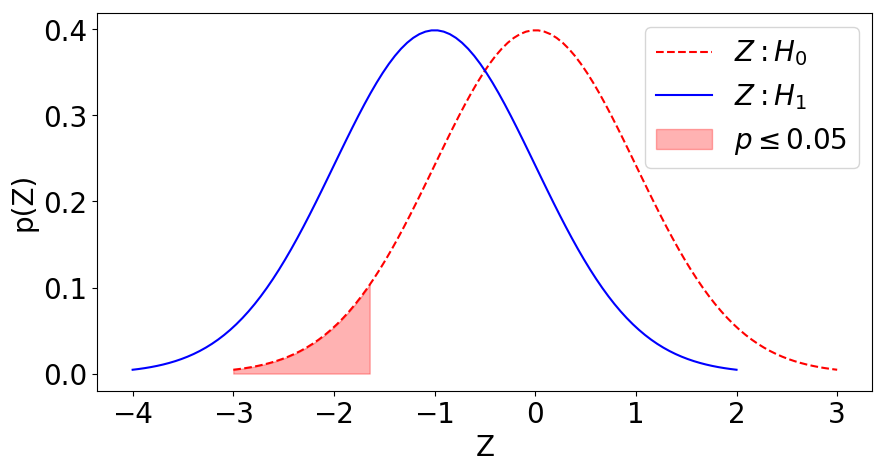
\includegraphics[width=0.5\textwidth]{z_less.png}
		\end{center}
	Достигаемый уровень значимости:
	$$p\left(Z\right) = 	F_{N(0,1)}(Z).
	$$
	}

	\only<3>{
		\begin{center}            
			\begin{tabular}{rl}
				выборка:                        & $X^n=\left(X_1,\ldots,X_n\right), X \sim N\left(\mu, \sigma^2\right)$\\
				& $\sigma$ известна         \\
				нулевая гипотеза:               & $H_0\colon \mu=\mu_0$ \\
				альтернатива:                   & $H_1\colon \mu > \mu_0$ \\
				статистика:                     & $Z\left(X^n\right) = \frac{\bar{X}-\mu_0}{\sigma / \sqrt{n}}$ \\
				нулевое распределение:          & $N(0,1)$\\
			\end{tabular}
			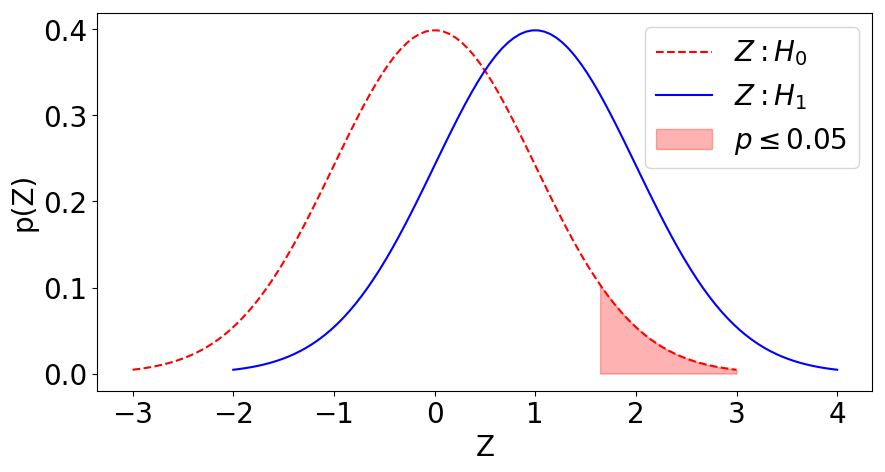
\includegraphics[width=0.5\textwidth]{z_more.png}
		\end{center}
	Достигаемый уровень значимости:
	$$p\left(Z\right) = 	1- F_{N(0,1)}(Z).
	$$
	}


	\only<4>{
        \large
        \begin{block}{Пример, Kanji, критерий 1}

		Линия по производству пудры должна обеспечивать средний вес пудры в упаковке 4 грамма, заявленное стандартное отклонение~--- 1 грамм. 
		
		В ходе инспекции выбрано 9 упаковок, средний вес продукта в них составляет 4.6 грамма.
		\end{block}
		\bigskip
		
		$H_0\colon$ средний вес пудры в упаковке соответствует норме.
		
		$H_1\colon$ средний вес пудры в упаковке не соответствует норме $\Rightarrow p = 0.0719,$ 95\% доверительный интервал для среднего веса~--- $\left[3.95, 5.25\right]$~г.
		
		$H_1\colon$ средний вес пудры в упаковке превышает норму  $\Rightarrow p = 0.0359,$ нижний 95\% доверительный предел для среднего веса~--- $4.05$~г.
        
    \textbf{Одностороннюю альтернативу можно использовать, если знак изменения среднего известен заранее.}

	}
\end{frame}

\begin{frame}[label=chitest1]{\hyperlink{onesample}{\beamerbutton{2}} Критерий хи-квадрат}
	\only<1>{
		\begin{center}
			\begin{tabular}{rl}
				выборка:                        & $X^n=\left(X_1,\ldots,X_n\right), X\sim N\left(\mu, \sigma^2\right)$  \\
				нулевая гипотеза:               & $H_0\colon \sigma=\sigma_0$ \\
				альтернатива:                   & $H_1\colon \sigma<\neq>\sigma_0$ \\
				статистика:                     & $\chi^2\left(X^n\right) = \frac{(n-1)S^2}{\sigma_0^2}$ \\
				нулевое распределение:          & $\chi^2_{n-1}$\\
			\end{tabular}
			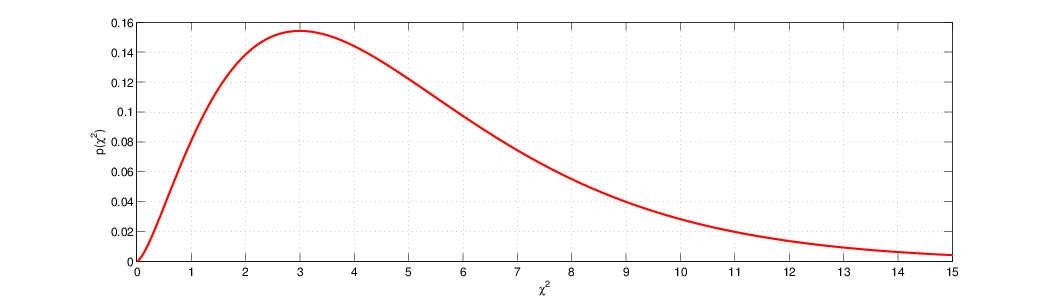
\includegraphics[width=0.7\textwidth]{chi2.png}   
		\end{center}
		достигаемый уровень значимости:
		$$p\left(\chi^2\right) = \begin{cases}
			1-F_{\chi^2_{n-1}}(\chi^2), 																  & H_1 \colon \sigma>\sigma_0, \\
			F_{\chi^2_{n-1}}(\chi^2),    																   & H_1 \colon \sigma<\sigma_0, \\
			2 \min\left( 1-F_{\chi^2_{n-1}}(\chi^2), F_{\chi^2_{n-1}}(\chi^2) \right),  & H_1 \colon \sigma\neq\sigma_0. \\
		\end{cases}$$
	}
	
	\only<2>{
    \large
    \begin{block}{Пример, Kanji, критерий 15}
		При производстве микрогидравлической системы делается инъекция жидкости. 
		Дисперсия объёма жидкости~--- критически важный параметр, установленный стандартом на уровне 9~кв.\,мл. 
		В выборке из 25~микрогидравлических систем выборочная дисперсия объёма жидкости составляет 12~кв.\,мл.
		     \end{block}	
		\bigskip
		
		$H_0\colon$ дисперсия объёма жидкости соответствует стандарту.
		
		$H_1\colon$ дисперсия объёма жидкости не соответствует стандарту $\Rightarrow p = 0.254,$ 95\% доверительный интервал для дисперсии~--- $\left[7.3, 23.2\right]$~кв.\,мл.
		
		$H_1\colon$ дисперсия объёма жидкости превышает допустимое значение $\Rightarrow p = 0.127,$ односторонний нижний 95\% доверительный предел~--- $7.9$~кв.\,мл.
   
}
\end{frame}

\begin{frame}[label=ttest1]{\hyperlink{onesample}{\beamerbutton{3}} t-критерий Стьюдента}
%%%%%%%%%%%%%%%%%%%%%%%%%%%%%%%%%%%%%%%%%%%%%%%%%%%%%%%%%%%%%%%%%%%%%
% Если дисперсия выборки неизвестна, вместо Z-критерия Стьюдента нужно применять t-критерий Стьюдента. Он основан на следующей идее: поскольку сигма неизвестна, то нужно в формуле статистики заменить сигма на S (выборочное стандартное отклонение). Такая статистика имеет уже не стандартное нормальное нулевое распределение, а распределение Стьюдента с числом степеней свободы n?1
% Чем больше объем выборки в задаче, тем меньше различий между t-критерием и Z-критерием. Это происходит по двум причинам: во-первых, чем больше n, тем точнее выборочная дисперсия S2 оценивает теоретическую дисперсию. Во-вторых, с ростом n увеличивается число степеней свободы у нулевого распределения t-критерия, а чем больше степеней свободы у распределения Стьюдента, тем больше оно похоже на стандартное нормальное. Ранее уже упоминалось, что, начиная с 30 степеней свободы, распределение Стьюдента визуально практически неотличимо от стандартного нормального. Благодаря этим двум фактам для достаточно больших выборок знание истинного значения дисперсии не оказывает большого влияния на результат.
%%%%%%%%%%%%%%%%%%%%%%%%%%%%%%%%%%%%%%%%%%%%%%%%%%%%%%%%%%%%%%%%%%%%%
	\only<1>{
		\begin{center}
			\begin{tabular}{rl}
				выборка:                        & $X^n=\left(X_1,\ldots,X_n\right), X \sim N\left(\mu, \sigma^2\right)$\\
				& $\sigma$ неизвестна         \\
				нулевая гипотеза:               & $H_0\colon \mu=\mu_0$ \\
				альтернатива:                   & $H_1\colon \mu<\neq>\mu_0$ \\
				статистика:                     & $T\left(X^n\right) = \frac{\bar{X}-\mu_0}{S / \sqrt{n}}$ \\
				нулевое распределение:          & $St(n-1)$\\
			\end{tabular}
			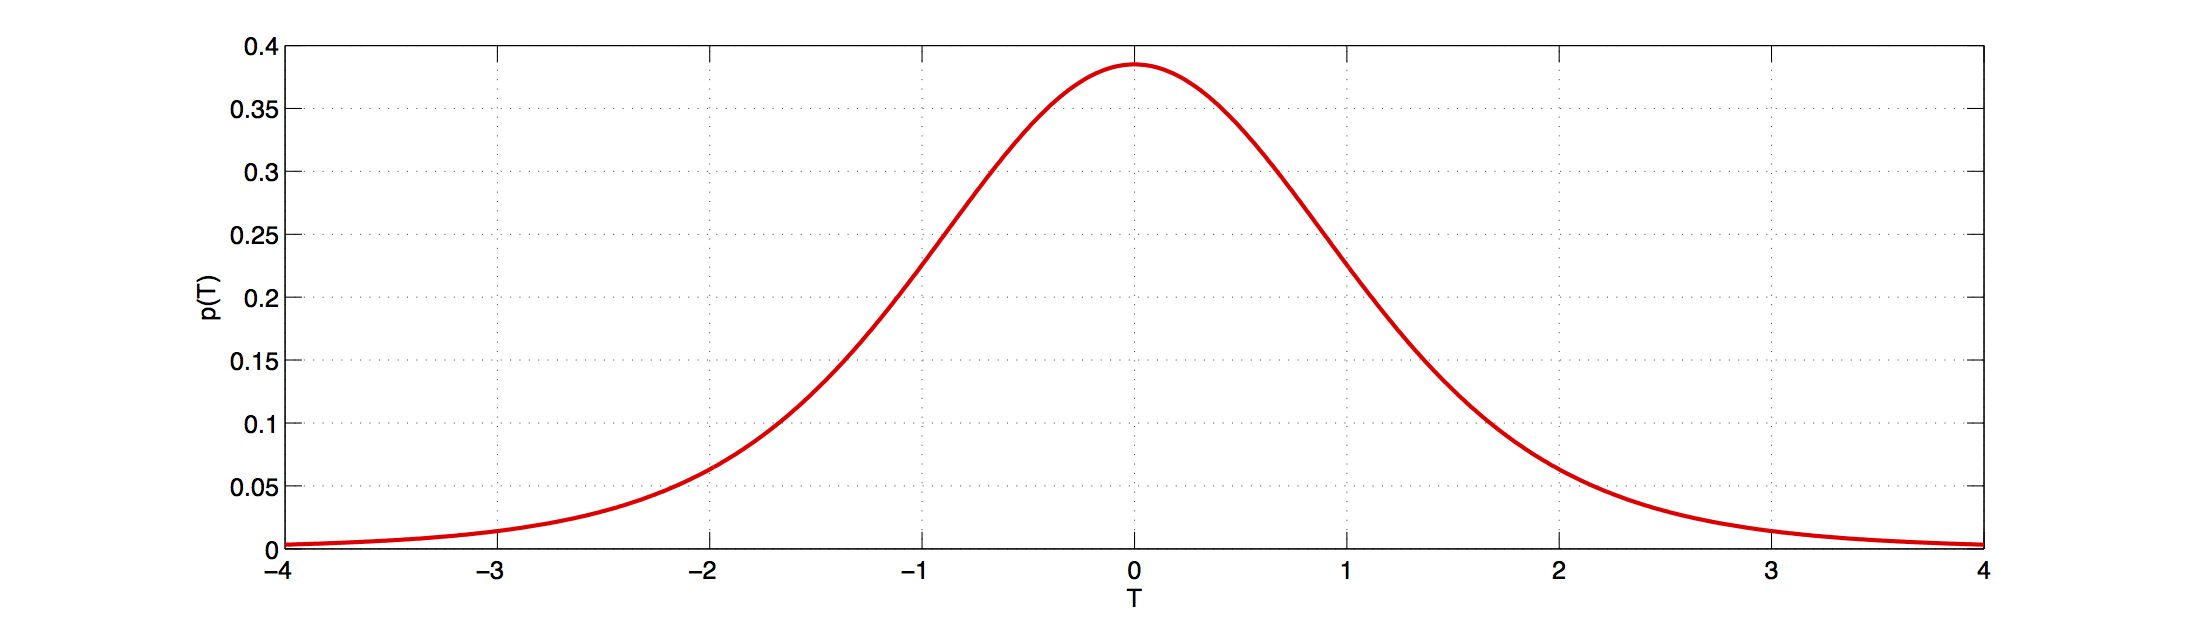
\includegraphics[width=0.7\textwidth]{stud.png}                
		\end{center}
		С ростом объёма выборки разница между t- и z-критериями уменьшается. 
	}
	
	\only<2>{
%%%%%%%%%%%%%%%%%%%%%%%%%%%%%%%%%%%%%%%%%%%%%%%%%%%%%%%%%%%%%%%%%%%%%%%
%%  Вес при рождении — это очень важный показатель здоровья ребенка. Так, только 7\% детей рождаются с весом меньше 2.5 кг, однако на них приходится 70\% детских смертей.
%%%%%%%%%%%%%%%%%%%%%%%%%%%%%%%%%%%%%%%%%%%%%%%%%%%%%%%%%%%%%%%%%%%%%%%% 

    \begin{block}{Пример}
	Cредний вес детей при рождении составляет 3300~г. В то же время, если мать ребёнка живёт за чертой бедности, то средний вес таких детей — 2800~г. 
	
	С целью увеличить вес тех детей, чьи матери живут за чертой бедности, разработана экспериментальная программа ведения беременности. Чтобы проверить ее эффективность, проводится эксперимент. В нём принимают участие 25~женщин, живущих за чертой бедности. У всех них рождаются дети, и их средний вес составляет 3075~г, выборочное стандартное отклонение~--- 500~г.
	
	Эффективна ли программа?
	     \end{block}	
	\bigskip
	
	$H_0\colon$ программа не влияет на вес детей, $\mu=2800$
	
	$H_1\colon$ программа как-то влияет на вес детей,  $\mu\neq2800 \Rightarrow p = 0.0111$, 95\% доверительный интервал для изменения веса~--- $\left[68.6, 481.4\right]$~г.
	
	$H_1\colon$ программа увеличивает вес детей,  $\mu>2800 \Rightarrow p = 0.0056$, 95\% нижний доверительный предел для увеличения веса~--- $103.9$~г.
	}
\end{frame}

\begin{frame}{Выбор альтернативы}
%%%%%%%%%%%%%%%%%%%%%%%%%%%%%%%%%%%%%%%%%%%%%%%%%%%%%%%%%%%%%%%%%%%%%%%
% Рассмотренный пример показывает, что, используя одностороннюю альтернативу вместо двусторонней, можно получить достигаемый уровень значимости в два раза меньше. В данной задаче это было не критично, поскольку оба достигаемых уровня значимости маленькие. Но иногда может оказаться, что p-value при двусторонней альтернативе больше магического порога в 0.05, а при односторонней альтернативе — меньше. То есть, используя одностороннюю альтернативу вместо двухсторонней, можно отвергнуть нулевую гипотезу. В таком случае кажется, что можно всегда использовать одностороннюю альтернативу, однако это нечестно. Альтернатива может быть односторонней только в некоторых случаях. Во-первых, если среднее должно изменится в какую-то определенную сторону и изменение в противоположную сторону невероятно. Во-вторых, направление изменения нужно определить до получения данных. Если односторонняя альтернатива выбирается после того, как данные получены, и она выбирается так, что ее знак соответствует знаку изменения выборочного среднего относительно mu0, то это — переобучение, и так делать нельзя.
%%%%%%%%%%%%%%%%%%%%%%%%%%%%%%%%%%%%%%%%%%%%%%%%%%%%%%%%%%%%%%%%%%%%%%%
\large
Одностороннюю альтернативу можно использовать, если знак изменения среднего известен заранее.

\bigskip

\textbf{Альтернатива должна выбираться до получения данных!}
\end{frame}


\subsection{Двухвыборочные задачи}
\begin{frame}[label=ztest2u]{\hyperlink{twosample}{\beamerbutton{4}} Z-критерий}
	\only<1>{
		\begin{center}
			\begin{tabular}{rl}
				выборки:                        & $X_1^{n_1}=\left(X_{11},\ldots,X_{1n_1}\right), X_{1} \sim N\left(\mu_1, \sigma_1^2\right)$ \\
				& $X_2^{n_2}=\left(X_{21},\ldots,X_{2n_2}\right), X_{2} \sim N\left(\mu_2, \sigma_2^2\right)$ \\
				& $\sigma_1, \sigma_2$ известны \\
				нулевая гипотеза:               & $H_0\colon \mu_1=\mu_2$ \\
				альтернатива:                   & $H_1\colon \mu_1<\neq>\mu_2$ \\
				статистика:                     & $Z\left(X_1^{n_1}, X_2^{n_2}\right) = \frac{\bar{X}_1-\bar{X}_2}{\sqrt{\frac{\sigma_1^2}{n_1}+\frac{\sigma_2^2}{n_2}}}$ \\
				нулевое распределение:          & $N(0,1)$\\
			\end{tabular}
			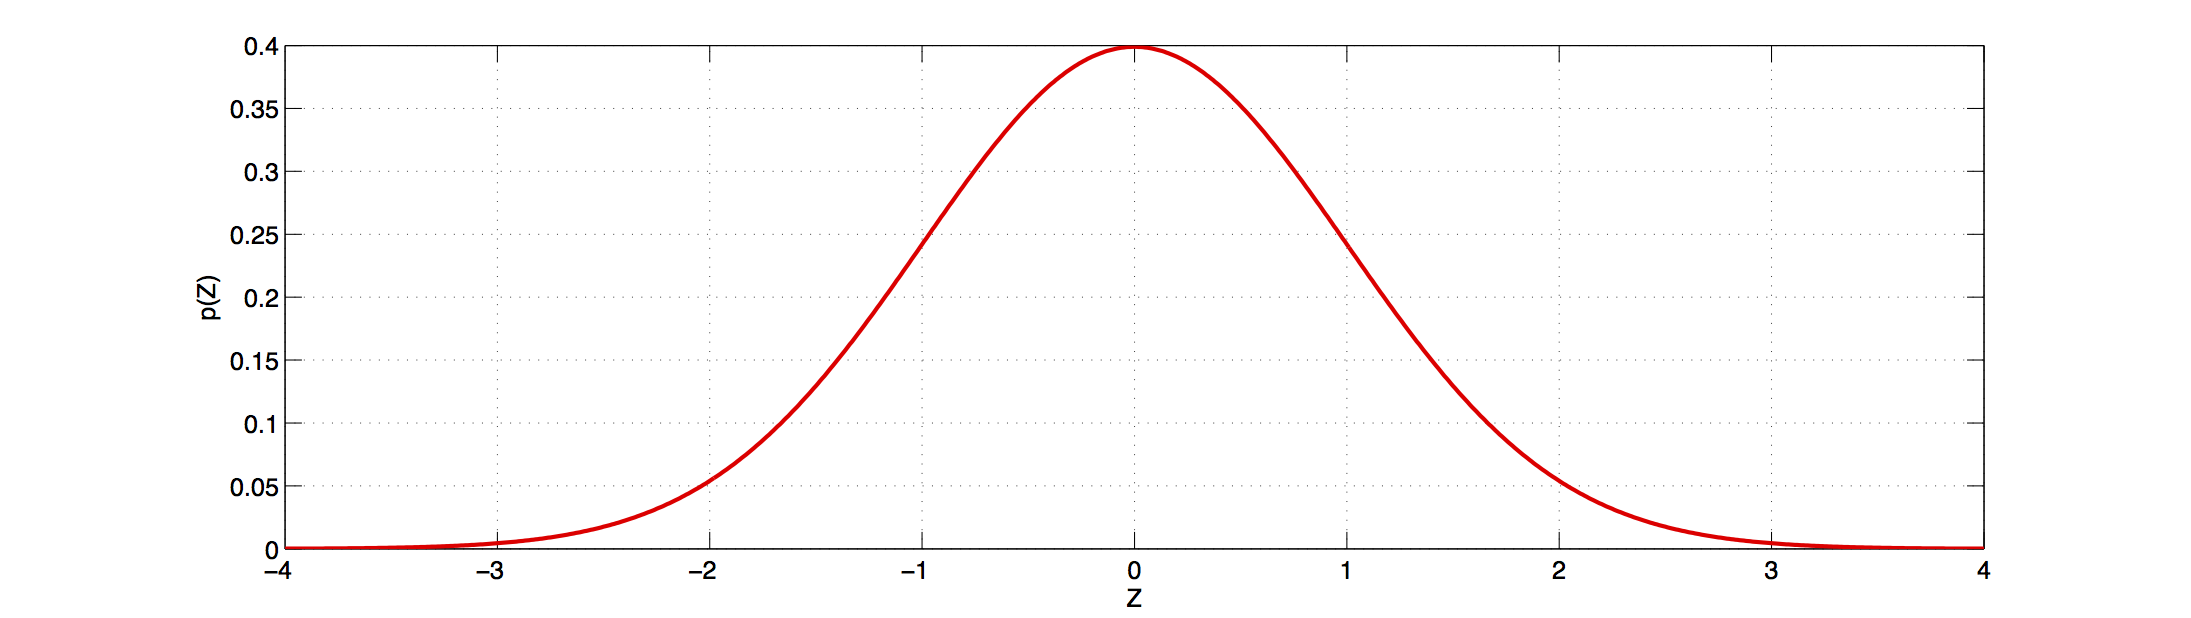
\includegraphics[width=0.7\textwidth]{norm.png}
		\end{center}
	}
	
	\only<2>{
    \large
    \begin{block}{Пример, Kanji, критерий 3}
 известно, что одна из линий по расфасовке чипсов даёт упаковки с более вариабельным весом продукта, чем вторая. Дисперсии равны 0.000576~$\text{г}^2$ и 0.001089~$\text{г}^2$ соответственно, средние значения веса в~выборках из~13 и~8~элементов~--- 80.02~г и 79.98~г.
		\end{block}
		\bigskip
		
		$H_0\colon$ средний вес продукта в упаковках, произведённых на двух линиях, совпадает.
		
		$H_1\colon$ средние веса продукта в упаковках, произведённых на двух линиях, различаются $\Rightarrow p = 0.001,$ 95\%~доверительный интервал для разности~--- $\left[0.039, 0.041\right]$.
	}
\end{frame}


\begin{frame}{Боксплот}
%%%%%%%%%%%%%%%%%%%%%%%%%%%%%%%%%%%%%%%%%%%%%%%%%%%%%%%%%%%%%%%%%%%%%%%
% Boxplot состоит из прямоугольника — ящика — и торчащих из него усов. Черта в середине прямоугольника соответствует выборочной медиане. Ширина ящика равна интерквартильному размаху, то есть, его нижняя граница — это 25%-й квантиль, а верхняя — 75%-й квантиль. Длина усов составляет 1.5 интерквартильных размаха, однако в разных реализациях кончик уса может рисоваться в разных местах. Так, на предыдущем слайде усы обрезаются так, что их конец соответствует последнему элементу выборки в этом направлении. Два кружочка на верхнем графике — это объекты выборки, не попавшие в диапазон 4 интерквартильных размаха.
%%%%%%%%%%%%%%%%%%%%%%%%%%%%%%%%%%%%%%%%%%%%%%%%%%%%%%%%%%%%%%%%%%%%%%%
	Ящик с усами~--- способ визуализации основных характеристик распределения:
	\begin{figure}
		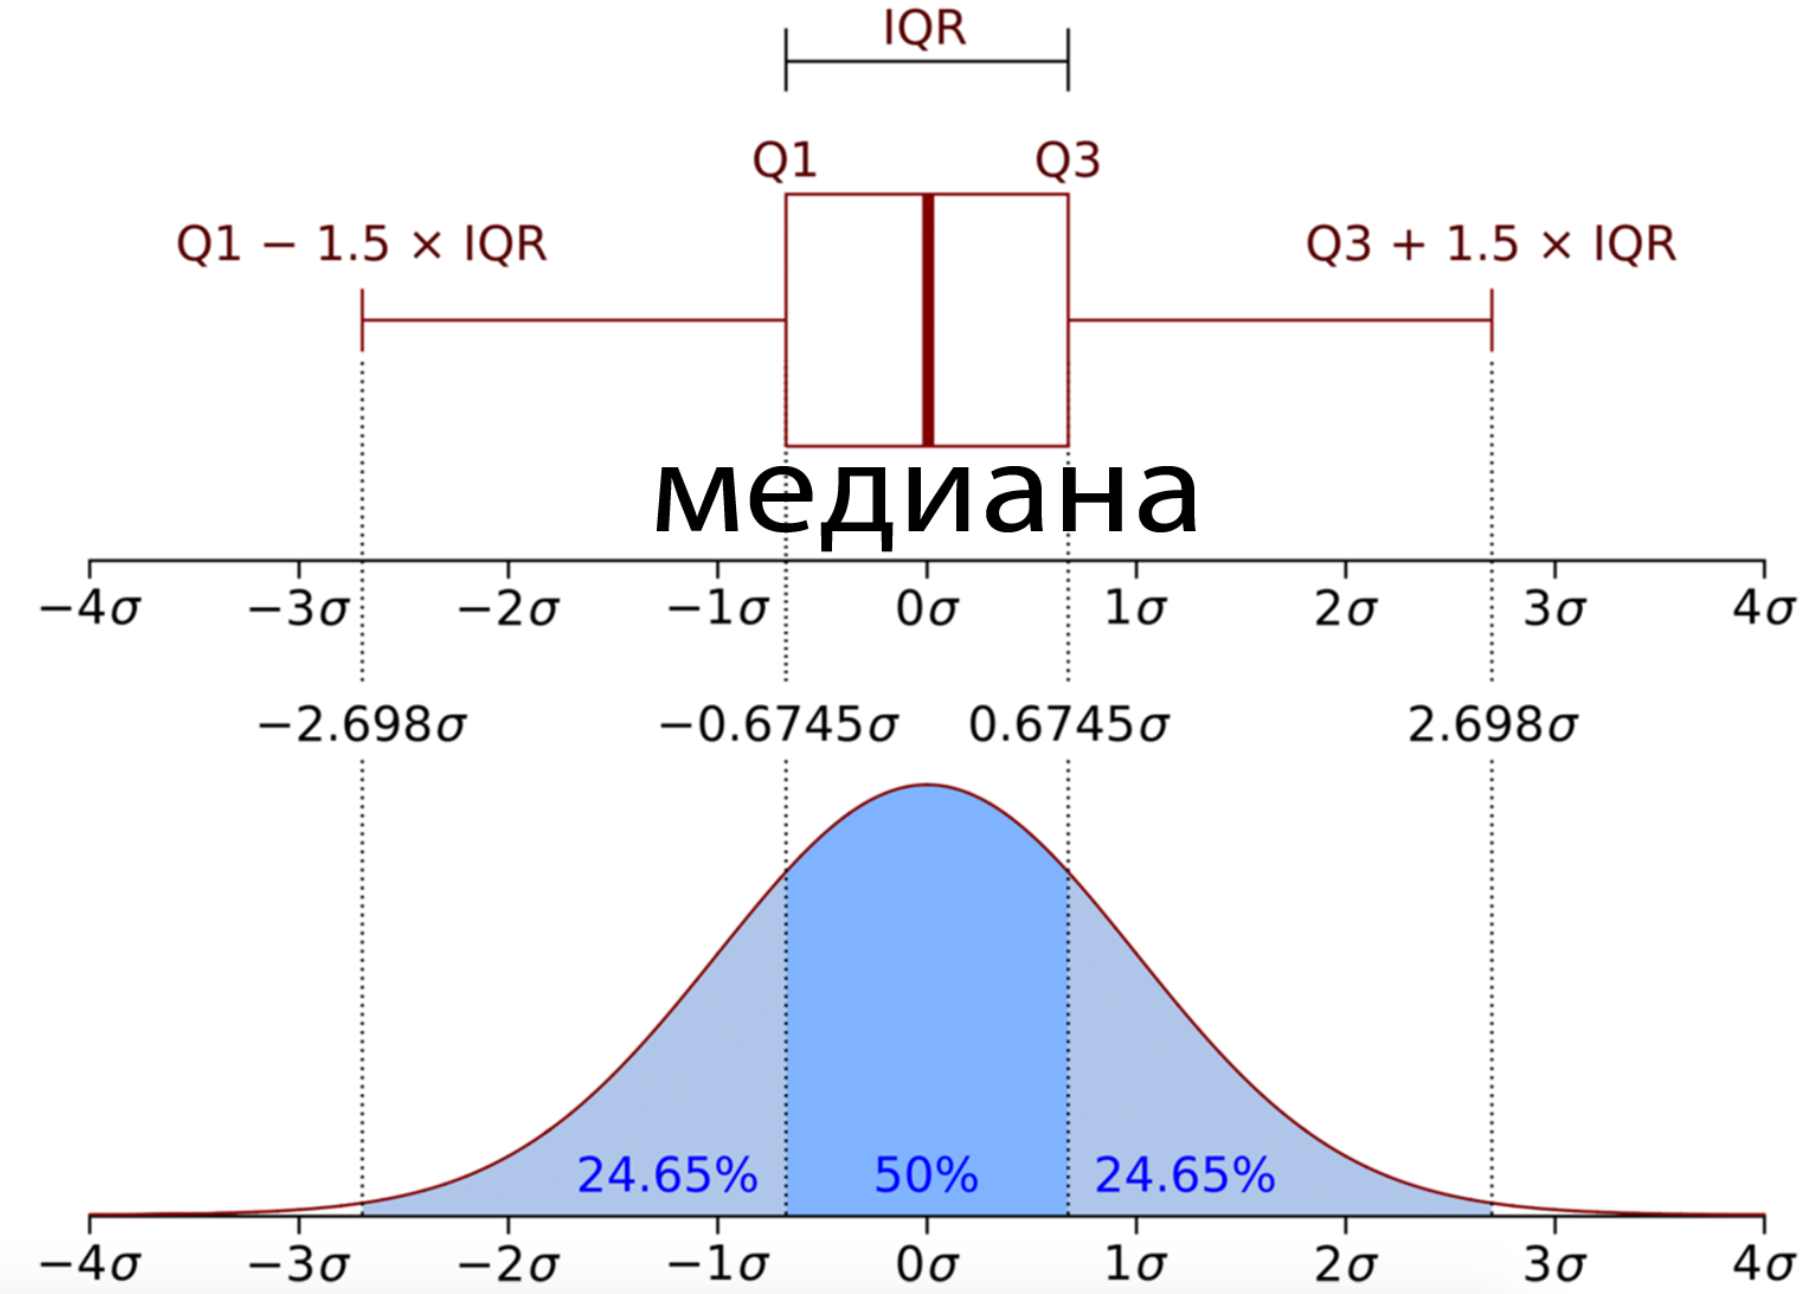
\includegraphics[width=0.7\textwidth]{boxplot.png}
	\end{figure} 
	Длина усов отличается в разных реализациях.
\end{frame}


\begin{frame}[label=ttest2u]{\hyperlink{twosample}{\beamerbutton{5}} t-критерий Стьюдента / Аспина-Уэлша (проблема Беренца-Фишера)}
	\only<1>{
%%%%%%%%%%%%%%%%%%%%%%%%%%%%%%%%%%%%%%%%%%%%%%%%%%%%%%%%%%%%%%%%%%%%%%%
% В более сложном случае дисперсии выборок неизвестны. Можно действовать по аналогии с одновыборочным случаем: в формуле для Z-критерия заменить все неизвестные сигмы на их выборочные оценки S1 и S2. Получится t-статистика.
% У этой задачи есть две проблемы. Во-первых, число степеней свободы ? у этого нулевого распределения Стьюдента вычисляется по достаточно сложной формуле. Во-вторых, нулевое распределение t-статистики не точное, а приближенное. Точного решения (то есть точного нулевого распределения для такой статистики) не существует. Эта проблема называется проблемой Беренца-Фишера: невозможно точно сравнить средние значение в двух выборках, дисперсии которых неизвестны.
% Однако рассмотренная аппроксимация достаточно точна в двух ситуациях. Во-первых, если выборки X1 и X2 одинакового объема, то есть n1 = n2. Во-вторых, если знак неравенства между n1 и n2 такой же, как между сигма1 и сигма2, то есть выборка с большей дисперсией по размеру не может быть меньше другой выборки. Если это условие выполнено, то можно использовать t-критерий Стьюдента и не переживать о точности аппроксимации. Если это не так, то возникает проблема: критерий Стьюдента перестает правильно работать, и вероятность ошибок первого рода начинает превышать уровень значимости ?. Это проблема не только критерия Стьюдента, она возникает при проверке любым способом гипотезы о равенстве средних в двух выборках с разной дисперсией. Поэтому, сравнивая средние значения в двух выборках, важно всегда следить за тем, чтобы выборка с большей дисперсией всегда была не меньшего объема, чем вторая выборка.
%%%%%%%%%%%%%%%%%%%%%%%%%%%%%%%%%%%%%%%%%%%%%%%%%%%%%%%%%%%%%%%%%%%%%%%
		\begin{center}
			\begin{tabular}{rl}
				выборки:                        & $X_1^{n_1}=\left(X_{11},\ldots,X_{1n_1}\right), X_{1}\sim N\left(\mu_1, \sigma_1^2\right)$ \\
				& $X_2^{n_2}=\left(X_{21},\ldots,X_{2n_2}\right), X_{2}\sim N\left(\mu_2, \sigma_2^2\right)$ \\
				& $\sigma_1, \sigma_2$ неизвестны \\
				нулевая гипотеза:               & $H_0\colon \mu_1=\mu_2$ \\
				альтернатива:                   & $H_1\colon \mu_1<\neq>\mu_2$ \\
				статистика:                     & $T\left(X_1^{n_1}, X_2^{n_2}\right) = \frac{\bar{X}_1-\bar{X}_2}{\sqrt{\frac{S_1^2}{n_1} + \frac{S_2^2}{n_2}}}$\\
				& $\nu = \frac{\left( \frac{S_1^2}{n_1} + \frac{S_2^2}{n_2} \right)^2}{ \frac{S_1^4}{n_1^2(n_1-1)} + \frac{S_2^4}{n_2^2(n_2-1)} }$ \\
				нулевое распределение:          & $\approx St(\nu)$\\
			\end{tabular}
			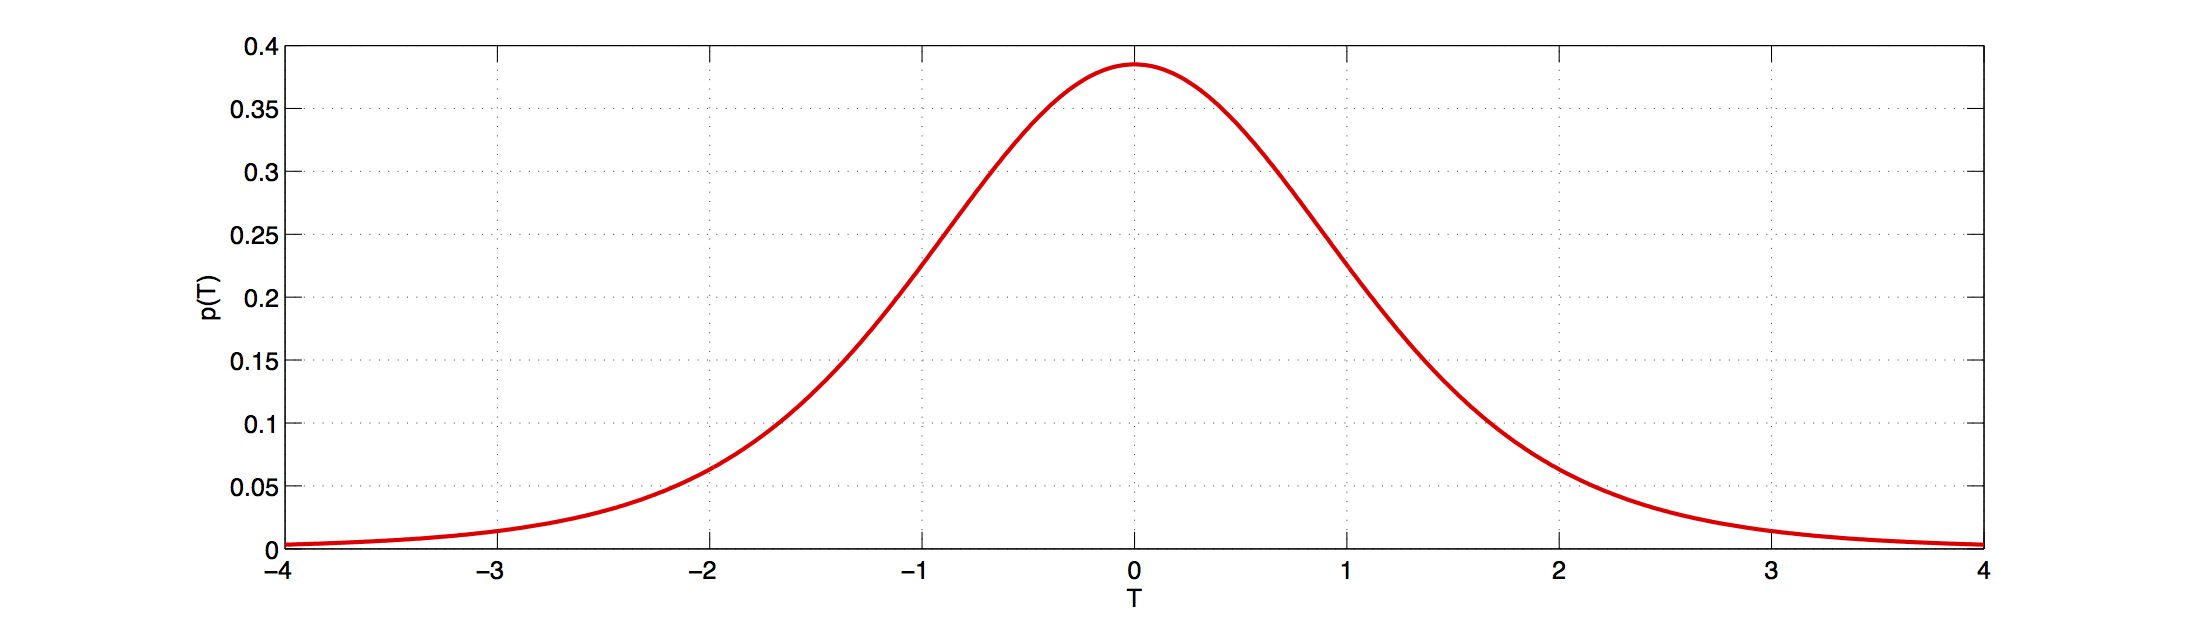
\includegraphics[width=0.7\textwidth]{stud.png}     
		\end{center}
		\textbf{Приближение достаточно точно при} $n_1=n_2$ \textbf{или} $\left[n_1>n_2\right] = \left[\sigma_1>\sigma_2\right].$
	}

\only<2>{
%%%%%%%%%%%%%%%%%%%%%%%%%%%%%%%%%%%%%%%%%%%%%%%%%%%%%%%%%%%%%%%%%%%%%%%
% General Social Survey. Это социологический опрос, который проводится на достаточно больших выборках в США уже больше 40 лет. В этом опросе очень много вопросов, которые задают респондентам, здесь будет рассматриваться только один.
%%%%%%%%%%%%%%%%%%%%%%%%%%%%%%%%%%%%%%%%%%%%%%%%%%%%%%%%%%%%%%%%%%%%%%%
	\small
    \begin{block}{Пример}
     В 1974 году 108 респондентов GSS работали неполный день, в 2014~--- 196. Для каждого из них известно количество рабочих часов за неделю, предшествующую опросу.

	\begin{figure}
		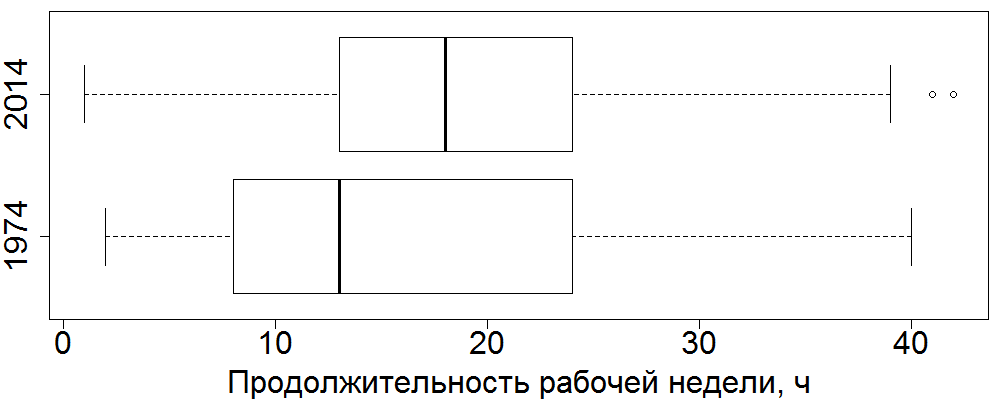
\includegraphics[width=0.75\textwidth]{hpw.png}
	\end{figure} 	
	Изменилось ли среднее время работы у работающих неполный день?
	\end{block}
	\bigskip

	$H_0\colon$ среднее время работы не изменилось, $\mu_1=\mu_2$.

	$H_0\colon$ среднее время работы изменилось, $\mu_1\neq\mu_2$.
	
	\bigskip
	
	t-критерий: $p=0.02707$, средняя продолжительность рабочей недели увеличилась на $2.57$~часов ($95$\% доверительный интервал~--- $\left[0.29, 4.85\right]$~ч).
	}
\end{frame}

\begin{frame}[label=ttest2p]{\hyperlink{twosample}{\beamerbutton{6}} t-критерий Стьюдента для связанных выборок}
	\only<1>{
%%%%%%%%%%%%%%%%%%%%%%%%%%%%%%%%%%%%%%%%%%%%%%%%%%%%%%%%%%%%%%%%%%%%%%%
% В числителе T-статистики стоит разность средних Х1 и X2. Это то же самое, что среднее X1 ? X2. Таким образом, t- критерий для двух связанных выборок эквивалентен одновыборочному t-критерию, примененному к выборке попарных разностей.
%%%%%%%%%%%%%%%%%%%%%%%%%%%%%%%%%%%%%%%%%%%%%%%%%%%%%%%%%%%%%%%%%%%%%%%
		\begin{center}
			\begin{tabular}{rl}
				выборки:                        & $X_1^{n}=\left(X_{11},\ldots,X_{1n}\right), X_{1} \sim N\left(\mu_1, \sigma_1^2\right)$ \\
				& $X_2^{n}=\left(X_{21},\ldots,X_{2n}\right), X_{2} \sim N\left(\mu_2, \sigma_2^2\right)$ \\
				& выборки связанные \\
				нулевая гипотеза:               & $H_0\colon \mu_1=\mu_2$ \\
				альтернатива:                   & $H_1\colon \mu_1<\neq>\mu_2$ \\
				статистика:                     & $T\left(X_1^{n}, X_2^{n}\right) = \frac{\bar{X}_1-\bar{X}_2}{S / \sqrt{n}}$\\
				& $S = \sqrt{ \frac1{n-1} \sum\limits_{i=1}^n \left(D_i-\bar{D}\right)^2 }$ \\
				& $D_i = X_{1i}-X_{2i}, \bar{D} = \frac{1}{n}\sum_i D_i$ \\
				нулевое распределение:          & $St(n-1)$\\
			\end{tabular}
			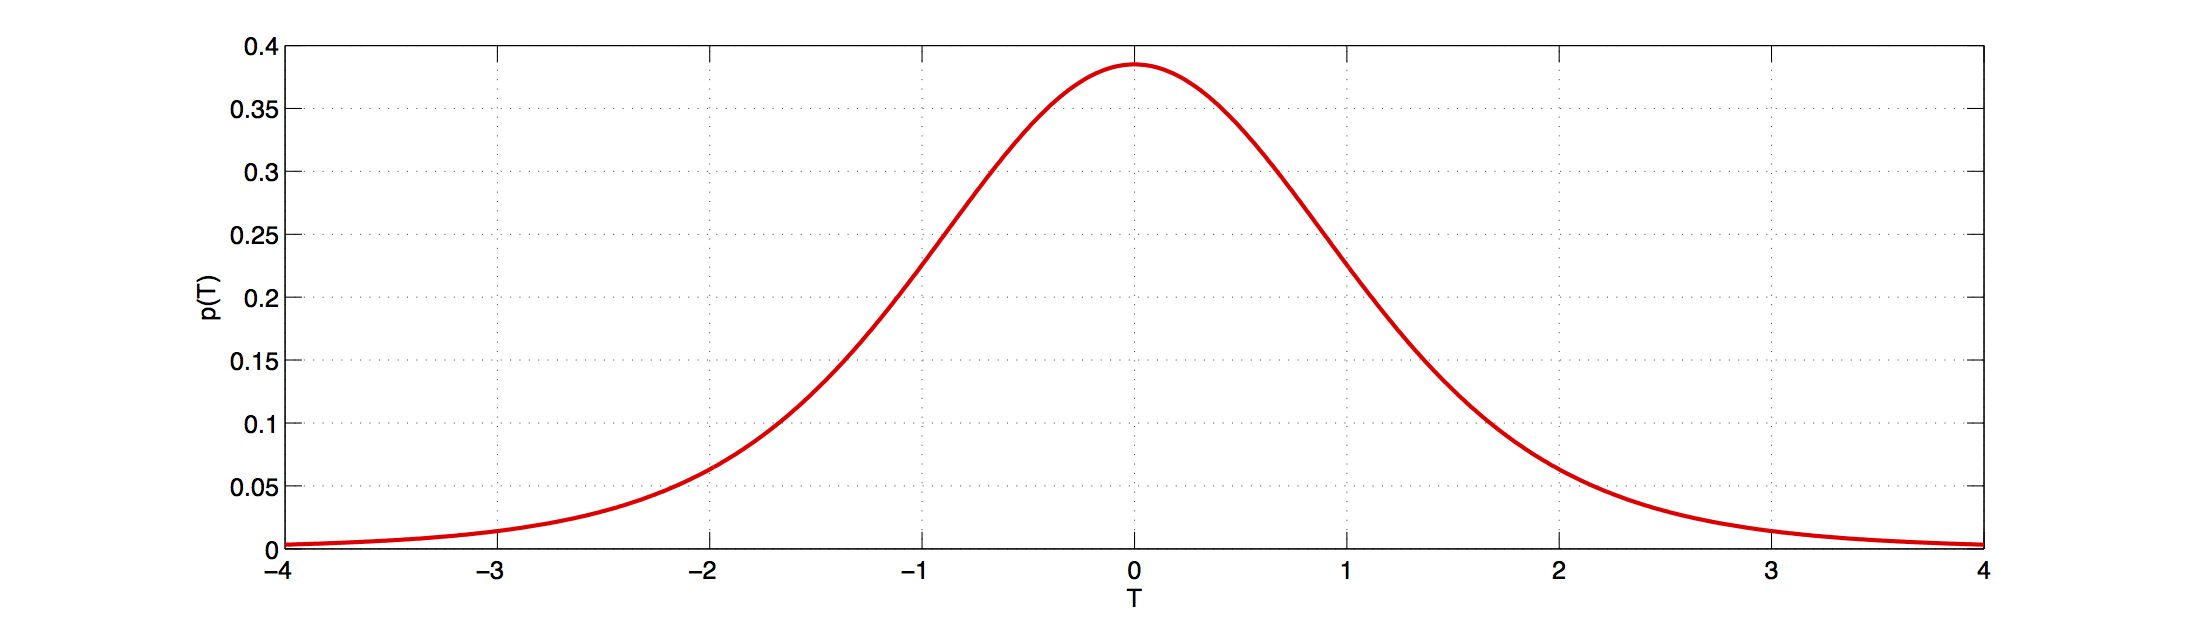
\includegraphics[width=0.7\textwidth]{stud.png}     
		\end{center}
	}
	
	\only<2>{
        \large
        \begin{block}{Пример, Kanji, критерий 10}
		На 10 испытуемых сравниваются два лекарства против респираторного заболевания. 
		Каждый из испытуемых вдыхает первое лекарство с помощью ингалятора, после чего проходит упражнение беговой дорожке.
		Измеряется время достижения максимальной нагрузки. 
		Затем после периода восстановления эксперимент повторяется со вторым лекарством.
		\end{block}
		\bigskip
		
		$H_0\colon$ время достижения максимальной нагрузки не отличается для исследуемых лекарств.
		
		\bigskip
		
		$H_1\colon$ время достижения максимальной нагрузки  для исследуемых лекарств отличается $ \Rightarrow  p=0.916;$  95\% доверительный интервал для разницы~--- $\left[-2.1, 0.9\right].$
	}
\end{frame}
	
	\begin{frame}{Пример}
		\only<1>{
            \begin{block}{}
			Пусть имеются следующие связные выборки:
			\begin{align*}
			X_1^n, & \;\; X_1\sim N(0,1), \\
			X_2^n, & \;\; X_2 = X_1 + \varepsilon, \;\; \varepsilon \sim N(0.1, 0.25) \Rightarrow X_2 \sim N(0.1, 1.25);
			\end{align*}
			требуется оценить разность $\Delta=\mathbb{E}X_1-\mathbb{E}X_2.$
			\end{block}

			1. Если \textbf{попарные соответствия элементов известны}, лучшая оценка $\hat{\Delta}_p = \frac1{n}\sum\limits_{i=1}^n\left(X_{1i}-X_{2i}\right)$ имеет дисперсию
			$$\mathbb{D}\hat{\Delta}_p = \frac1{n^2}\sum_{i=1}^n \mathbb{D}\left(X_{1i} - X_{2i}\right) = \frac1{n} \mathbb{D}\varepsilon = \frac1{2n};$$
			мощность 0.8 достигается при $n\approx200$.
			
			2. Если же \textbf{попарные соответствия неизвестны}, лучшая оценка~---  $\hat{\Delta}_i = \bar{X}_1 - \bar{X}_2$; её дисперсия:
			
			$$\mathbb{D}\hat{\Delta}_i = \frac1{n^2}\sum_{i=1}^n \mathbb{D}X_{1i} + \frac1{n^2}\sum_{i=1}^n \mathbb{D}X_{2i} = \frac1{n} + \frac{5}{4n} = \frac{9}{4n}$$
			--- в 4.5 раза больше; мощность 0.8 достигается при $n\approx1900$.	
		}
	\end{frame}
	
	\begin{frame}[label=ftest]{\hyperlink{twosample}{\beamerbutton{7}} F-критерий Фишера}
		\only<1>{
			\begin{center}
				\begin{tabular}{rl}
					выборки:                        & $X_1^{n_1}=\left(X_{11},\ldots,X_{1n_1}\right), X_{1} \sim N\left(\mu_1, \sigma_1^2\right)$ \\
					& $X_2^{n_2}=\left(X_{21},\ldots,X_{2n_2}\right), X_{2} \sim N\left(\mu_2, \sigma_2^2\right)$ \\
					нулевая гипотеза:               & $H_0\colon \sigma_1=\sigma_2$ \\
					альтернатива:                   & $H_1\colon \sigma_1<\neq>\sigma_2$ \\
					статистика:                     & $F\left(X_1^{n_1}, X_2^{n_2}\right) = \frac{S_1^2}{S_2^2}$ \\
					нулевое распределение:          & $F(n_1-1, n_2-1)$\\
				\end{tabular}
				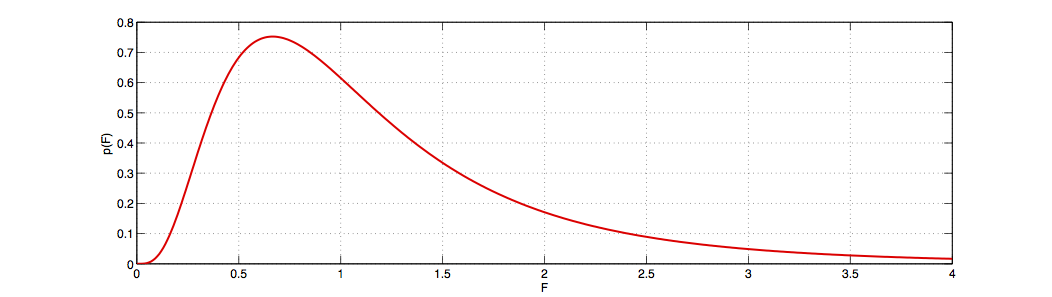
\includegraphics[width=0.7\textwidth]{fish.png}
			\end{center}
			Критерий Фишера неустойчив к отклонениям от нормальности даже асимптотически.
		}
		
		\only<2>{
            \begin{block}{Пример, NIST/industry ceramics consortium for strength optimization of ceramic, 1996} 
        Собраны данные о прочности материала 440~керамических изделий из двух партий по 220 в каждой. 
			
			Одинакова ли дисперсия прочности в разных партиях?
	\end{block}
			\begin{center}
				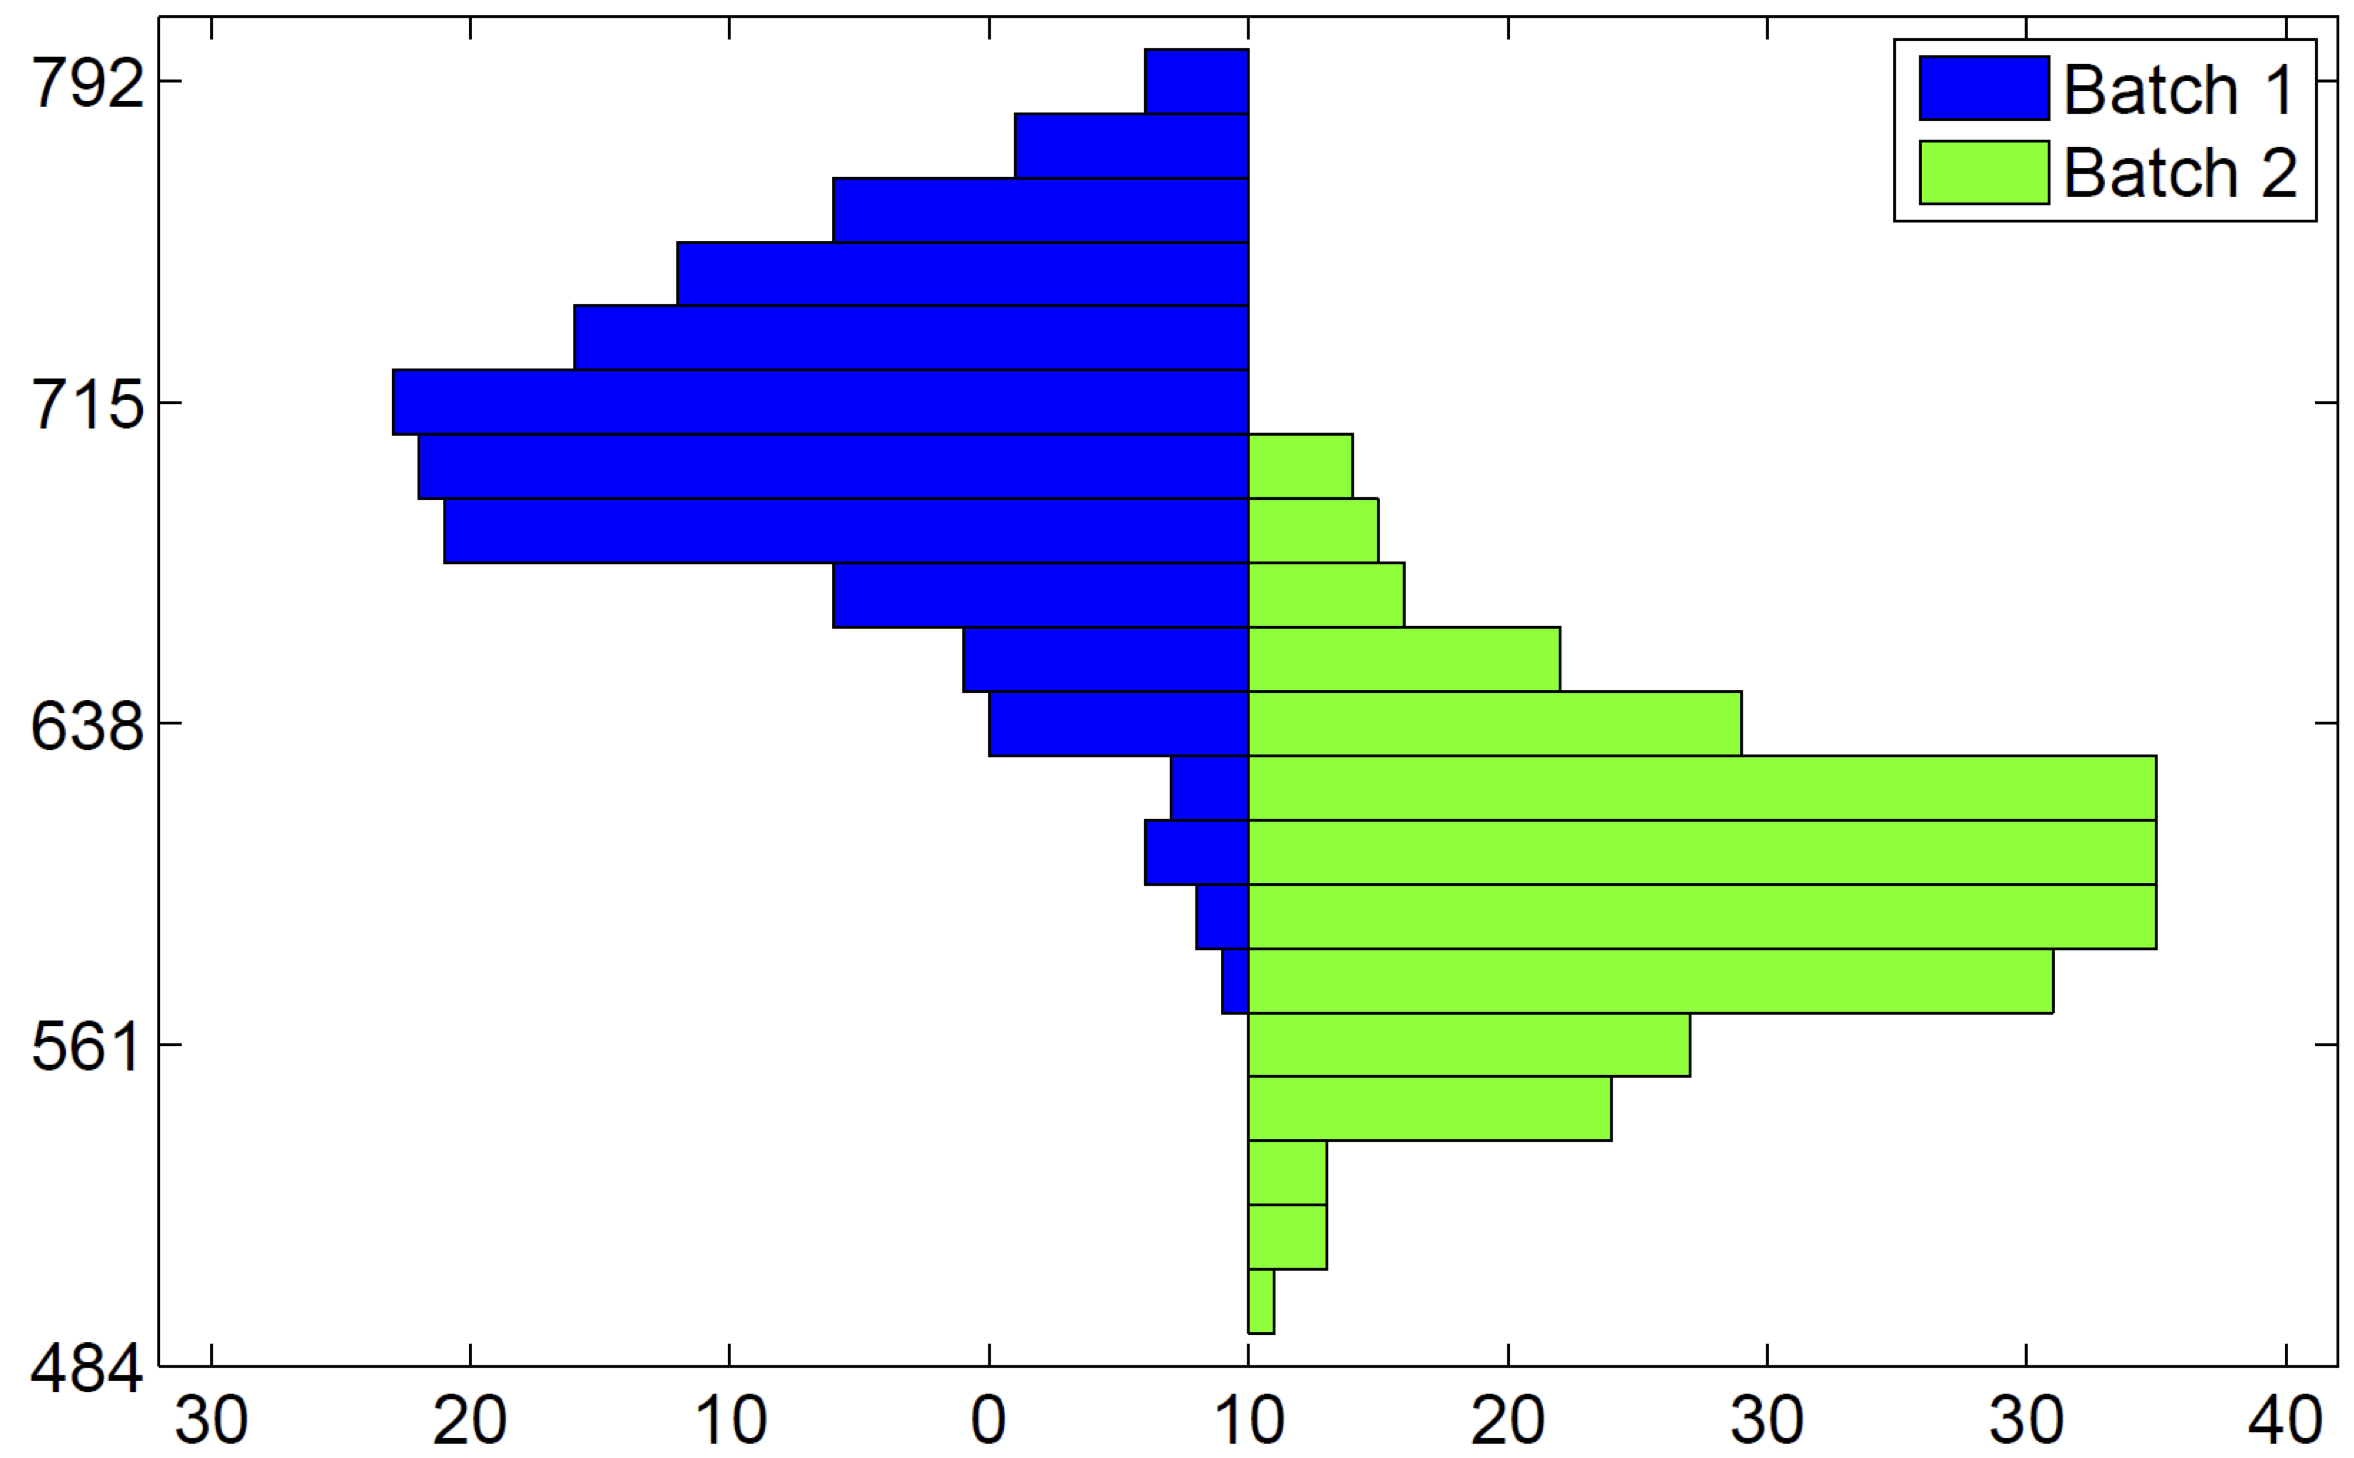
\includegraphics[width=0.7\textwidth]{ceramics.png}
			\end{center}
%			\
%			Гипотезы нормальности не отклоняются критерием Шапиро-Уилка ($p_1=0.2062, p_2=0.7028$).
		
			Критерий Фишера: $p=0.1721, \;\; \left[C_L, C_U\right]=\left[0.9225, 1.5690\right].$
		}
	\end{frame}

\subsection{Проверка нормальности}
\begin{frame}{Коэффициент ассиметрии}
\begin{itemize}
	\item \textbf{коэффициент ассиметрии} (skewness):
	\end{itemize}
	$$\gamma_1 = \mathbb{E} \left( \frac{X-\mathbb{E}X} {\sqrt{\mathbb{D}X}} \right)^3$$
	\begin{center}
		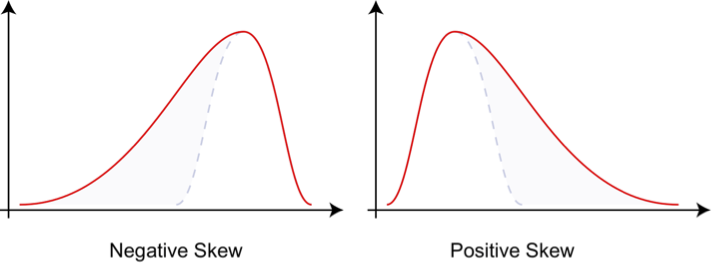
\includegraphics[width=\textwidth]{skewness.png}
	\end{center}
	
\end{frame}

\begin{frame}{Коэффициент экцесса}
\begin{itemize}
			\item \textbf{коэффициент эксцесса} (excess, без вычитания тройки~--- kurtosis):
		\end{itemize}
	$$\gamma_2 =  \frac{\mathbb{E}\left(X-\mathbb{E}X\right)^4}{\left(\mathbb{D}X\right)^2} - 3$$
	\begin{center}
		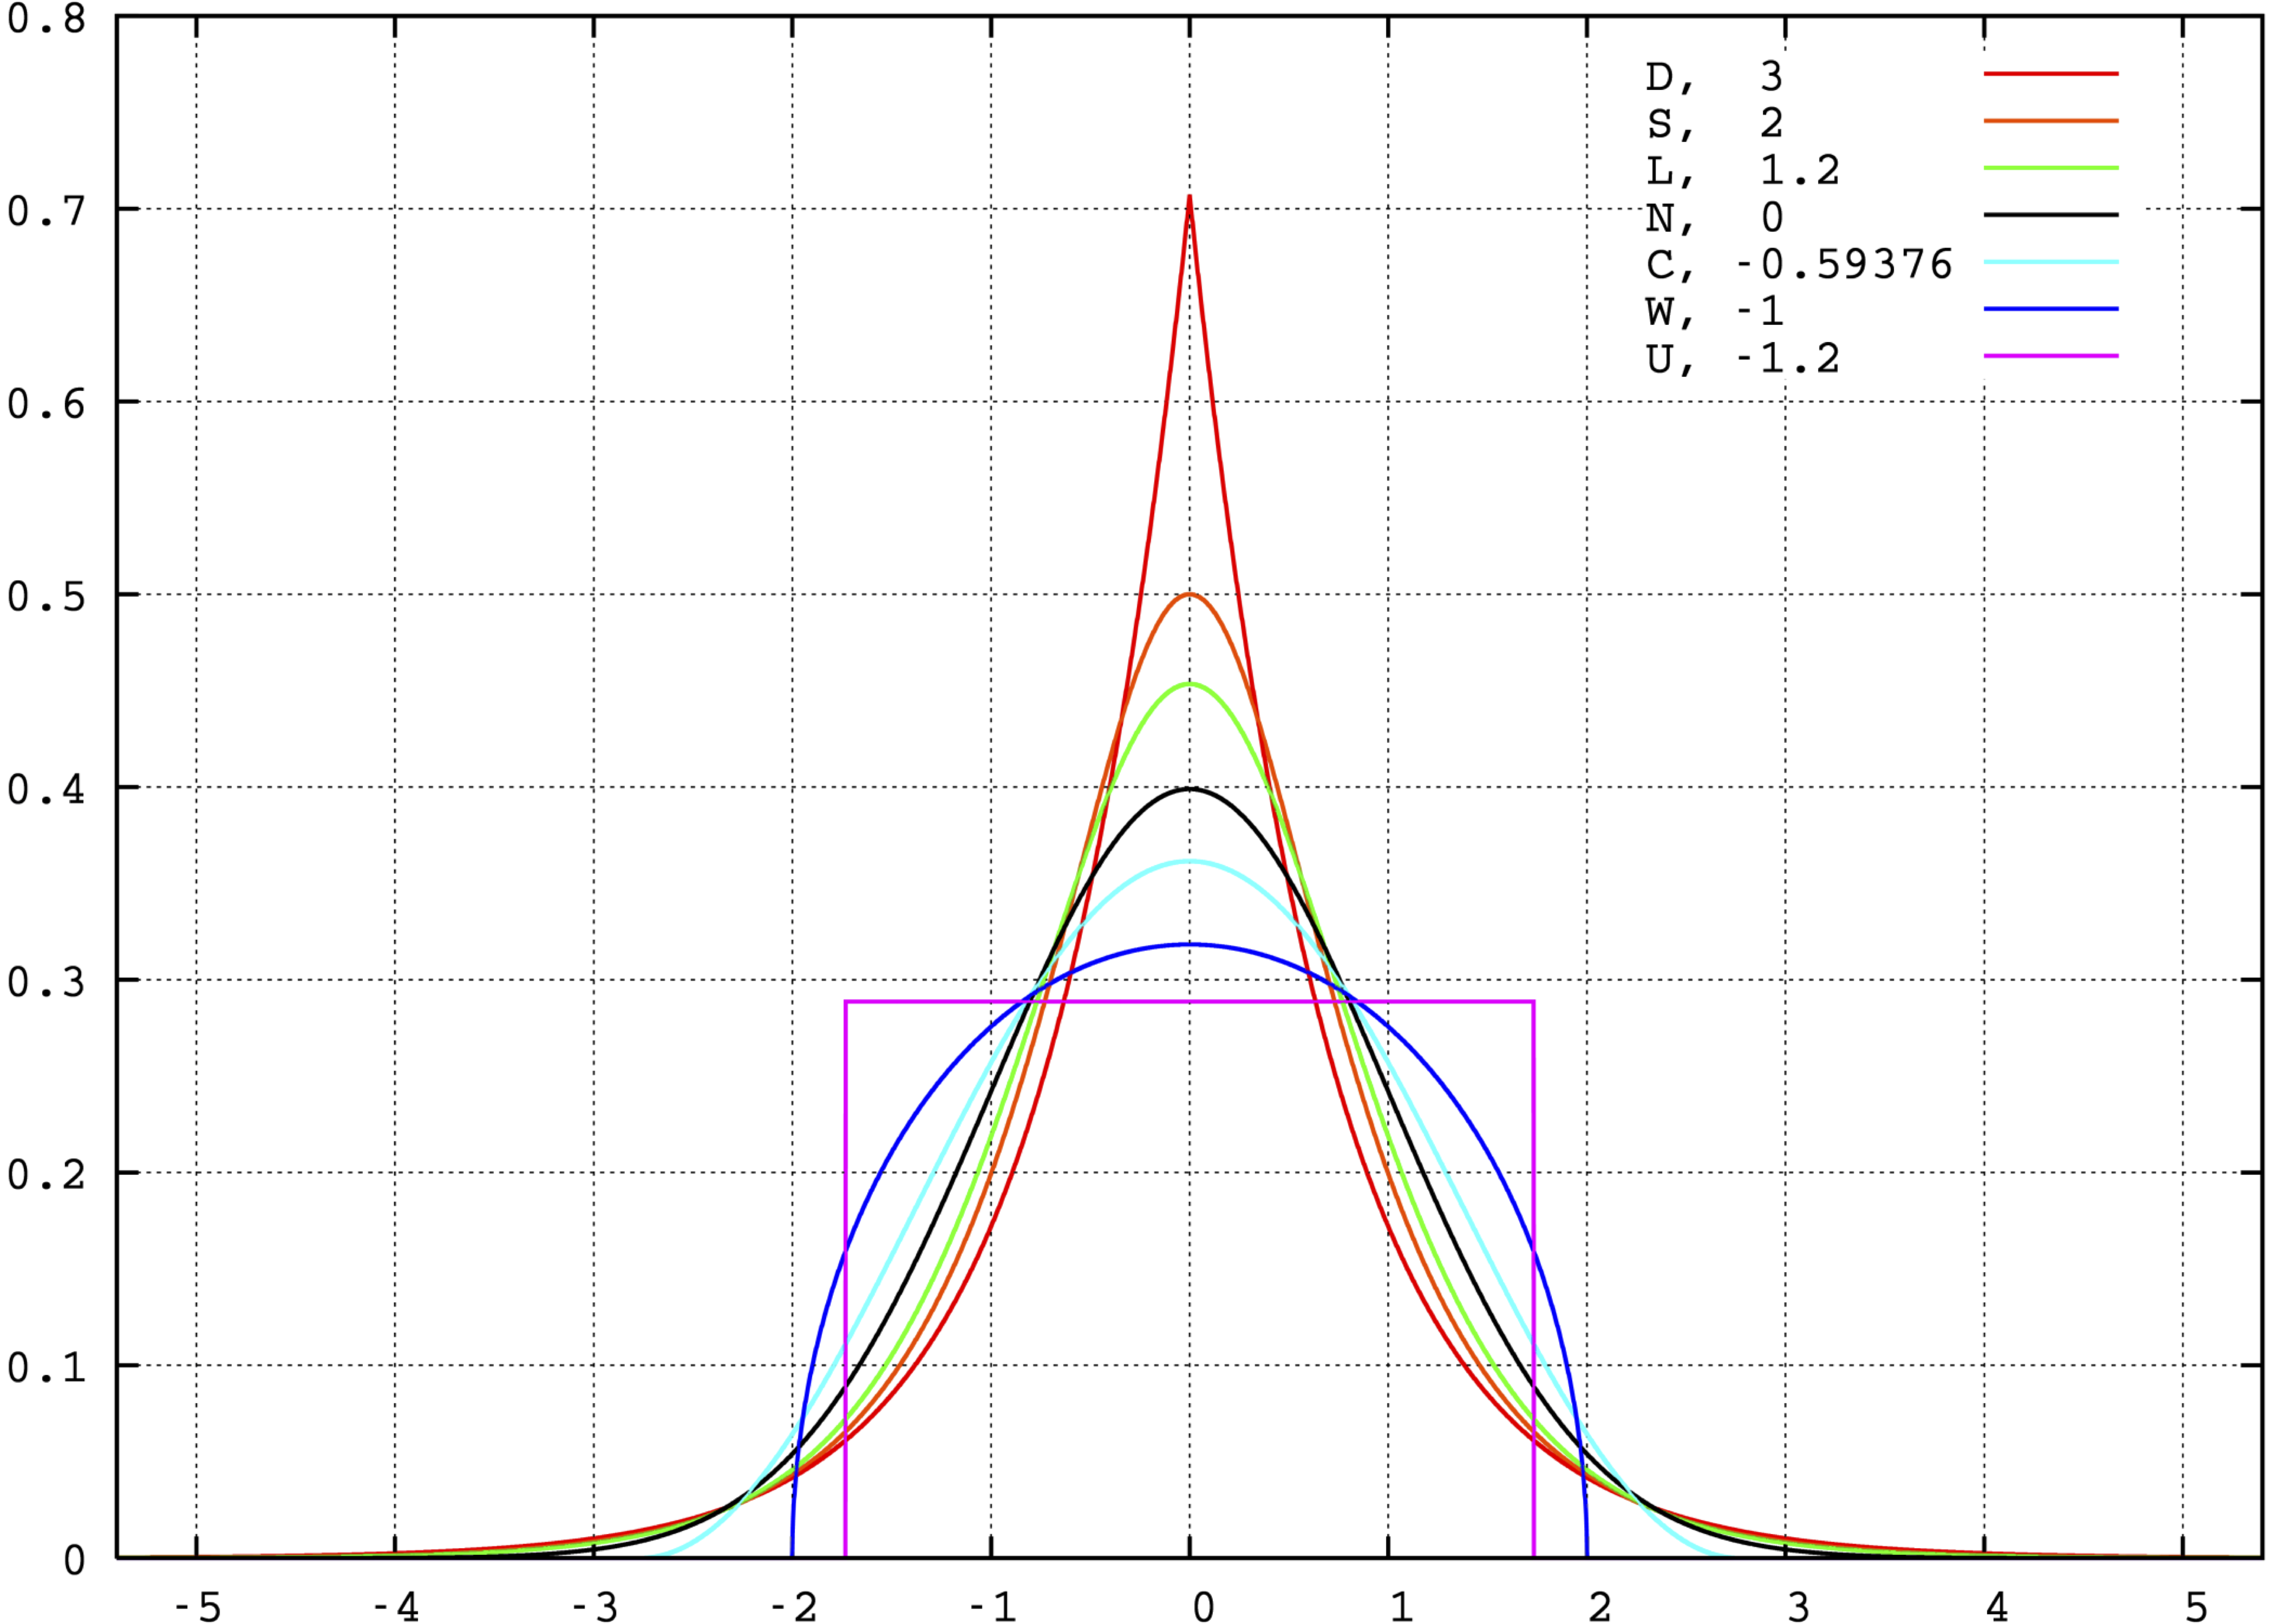
\includegraphics[width=0.6\textwidth]{kurtosis.png}
	\end{center}
	
\end{frame}
\begin{frame}{Критерий Харке-Бера}
	\begin{center}
		\begin{tabular}{rl}
			выборка:                        & $X^n=\left(X_1,\ldots,X_n\right)$         \\
			нулевая гипотеза:               & $H_0\colon X \sim N\left(\mu,\sigma^2\right)$ \\
			альтернатива:                   & $H_1\colon H_0$ неверна \\
			статистика:                     & $\chi^2\left(X^n\right) = \frac{n}{6}\left(\gamma_1^2 + \frac1{4} \gamma_2^2\right)$ \\
			нулевое распределение:          & $\chi^2_2$\\
		\end{tabular}
		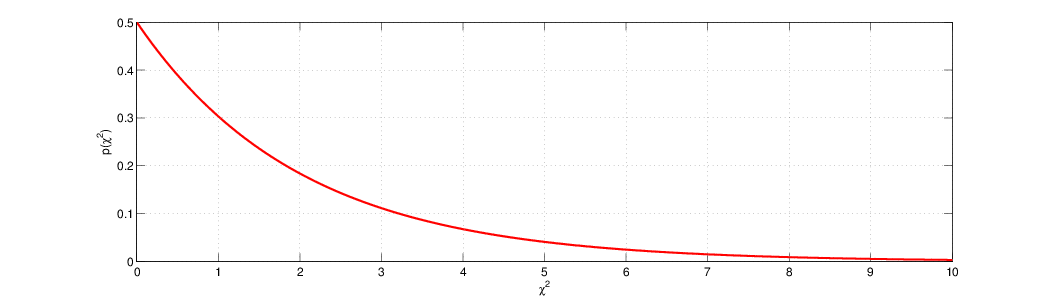
\includegraphics[width=0.7\textwidth]{chi22.png}
	\end{center}
	достигаемый уровень значимости:
	$$p\left(\chi^2\right) = 1 - F_{\chi^2_2}\left(\chi^2\right)$$
\end{frame}

\begin{frame}{Критерий согласия Пирсона (хи-квадрат)}   
%%%%%%%%%%%%%%%%%%%%%%%%%%%%%%%%%%%%%%%%%%%%%%%%%%%%%%%%%%%%%%%%%%%%%%%
% Статистика критерия конструируется следующим образом: область изменения случайной величины разбивается на K интервалов (карманов). Границы этих интервалов задаются величинами ai. Для каждого интервала [ai,ai+1] вычисляются две величины. Во-первых, ni — число элементов выборки, которое попало в интервал. Во-вторых, pi — теоретическая вероятность попадания в этот интервал при условии справедли- вости нулевой гипотезы. В данном случае это разность функций нормального распределения в точках ai+1 и ai
%%%%%%%%%%%%%%%%%%%%%%%%%%%%%%%%%%%%%%%%%%%%%%%%%%%%%%%%%%%%%%%%%%%%%%%
	\small{
		\begin{center}
			\begin{tabular}{rl}
				выборка:                        & $X^n=\left(X_1,\ldots,X_n\right)$         \\
				нулевая гипотеза:               & $H_0\colon X \sim N\left(\mu,\sigma^2\right)$ \\
				альтернатива:                   & $H_1\colon H_0$ неверна\\
				статистика:                     & $\chi^2\left(X^n\right) = \sum\limits_{i=1}^K \frac{\left(n_i - np_i\right)^2}{np_i}$ \\
				& $[a_i,a_{i+1}], i=1,\dots,K$ --- интервалы гистограммы \\                                            
				& $n_i$ --- число элементов выборки в $[a_i,a_{i+1}]$ \\                                
				& $p_i = F\left(a_{i+1}\right) - F\left(a_i\right)$ --- вероятность попадания \\
				& в $i$-й интервал при $H_0$\\
				нулевое распределение:          & $\begin{cases}
				\chi^2_{K-1}, & \mu, \sigma \text{ заданы,} \\
				\chi^2_{K-3}, & \mu, \sigma \text{ оцениваются},
				\end{cases}$\\
			\end{tabular}
			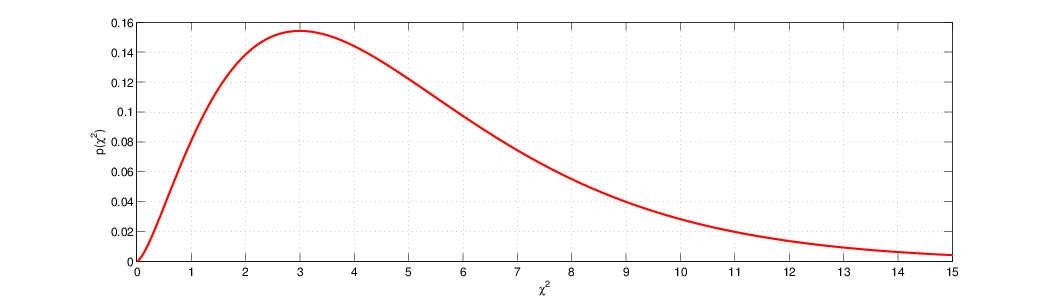
\includegraphics[width=0.7\textwidth]{chi2.png}        
		\end{center}
		
		\vspace{-5pt}
		
		\textbf{Недостатки:}
		\begin{itemize}
			\item разбиение на интервалы неоднозначно
			\item требует больших выборок ($np_i>5$ в~80\%~ячеек)
		\end{itemize}
	}
\end{frame}

\begin{frame}{Критерии, основанные на эмпирической функции распределения}
	\only<1>{
		Ряд критериев согласия основаны на различиях между $F\left(x\right)$ и $F_n\left(x\right)$:
		\begin{itemize}
			\item Джини: $$\int\left|F_n\left(x\right)-F\left(x\right)\right|dx$$
			\item Крамера-фон Мизеса: $$\int\left(F_n\left(x\right)-F\left(x\right)\right)^2dx$$
			\item Колмогорова (одновыборочный Колмогорова-Смирнова): $$\sup_{-\infty<x<\infty}\left|F_n\left(x\right)-F\left(x\right)\right|$$
			\item Смирнова-Крамера-фон Мизеса: $$\int\left(F_n\left(x\right)-F\left(x\right)\right)^2dF\left(x\right)$$
		\end{itemize}
	}
	
	\only<2>{
		\begin{itemize}
			\item Андерсона-Дарлинга: $$\int\frac{\left(F_n\left(x\right)-F\left(x\right)\right)^2}{F\left(x\right) \left(1-F\left(x\right)\right)}dF\left(x\right)$$
			\item Купера: $$\sup_{-\infty<x<\infty}\left(F_n\left(x\right)-F\left(x\right)\right) + \sup_{-\infty<x<\infty}\left(F\left(x\right)-F_n\left(x\right)\right)$$
			\item Ватсона: $$\int\left(F_n\left(x\right)-F\left(x\right) - \int \left(F_n\left(x\right)-F\left(x\right)\right)dF\left(x\right) \right)dF\left(x\right)$$
			\item Фроцини: $$\int\left|F_n\left(x\right)-F\left(x\right)\right|dF\left(x\right)$$
		\end{itemize}
		
		Предполагается, что $F\left(x\right)$ известна с точностью до параметров (если они оцениваются по выборке, нулевое распределение корректируется).
	}
\end{frame}

\begin{frame}{Критерий Колмогорова (Лиллиефорса)}
	\begin{center}
		\begin{tabular}{rl}
			выборка:                        & $X^n=\left(X_1,\ldots,X_n\right)$         \\
			нулевая гипотеза:               & $H_0\colon X \sim N\left(\mu,\sigma^2\right)$ \\
			альтернатива:                   & $H_1\colon H_0$ неверна \\
			статистика:                     & $D\left(X^n\right) = \sup\limits_{-\infty<x<\infty} \left|F_n(x) - \Phi(x)\right|$ \\
			нулевое распределение:          & табличное\\
		\end{tabular}
	\end{center}
	
	\bigskip
	Недостатки:
	\begin{itemize}
		\item имеет низкую мощность
		\item не чувствителен к различиям на хвостах распределений
	\end{itemize}
\end{frame}


\begin{frame}{Q-Q plot}
	\only<1>{
%%%%%%%%%%%%%%%%%%%%%%%%%%%%%%%%%%%%%%%%%%%%%%%%%%%%%%%%%%%%%%%%%%%%%%%
% Чтобы построить такой график, выборку нужно превратить в вариационный ряд, то есть отсортировать по неубыванию, а дальше каждому объекту выборки сопоставить точку на графике. Значение по вертикальной оси соответствует значению X, а значение по горизонтальной оси — математическому ожиданию квантиля стандартного нормального распределения, посчитанного по выборке такого объема.
% Чтобы это лучше понять, можно посмотреть на точку в нижнем левом углу. Эта точка соответствует наименьшему значению в выборке. Пусть объе?м выборки — 100. Таким образом, эта точка — это минимум из всех 100 элементов. Значение этого минимума отложено по вертикальной оси. По горизонтальной оси отложено математическое ожидание минимума из 100 независимых одинаково распределенных случайных величин из стандартного нормального распределения. Если выборка взята из нормального распределения, точки на Q-Q графике должны лежать примерно на прямой. Если точки лучше описываются нелинейной кривой или какие-то из точек лежат от прямой очень далеко, скорее всего, распределение отличается от нормального.
%%%%%%%%%%%%%%%%%%%%%%%%%%%%%%%%%%%%%%%%%%%%%%%%%%%%%%%%%%%%%%%%%%%%%%%
		Визуальный метод проверки согласия выборки и распределения~--- q-q plot (для нормального распределения называется также normal probability plot)
		\begin{center}
			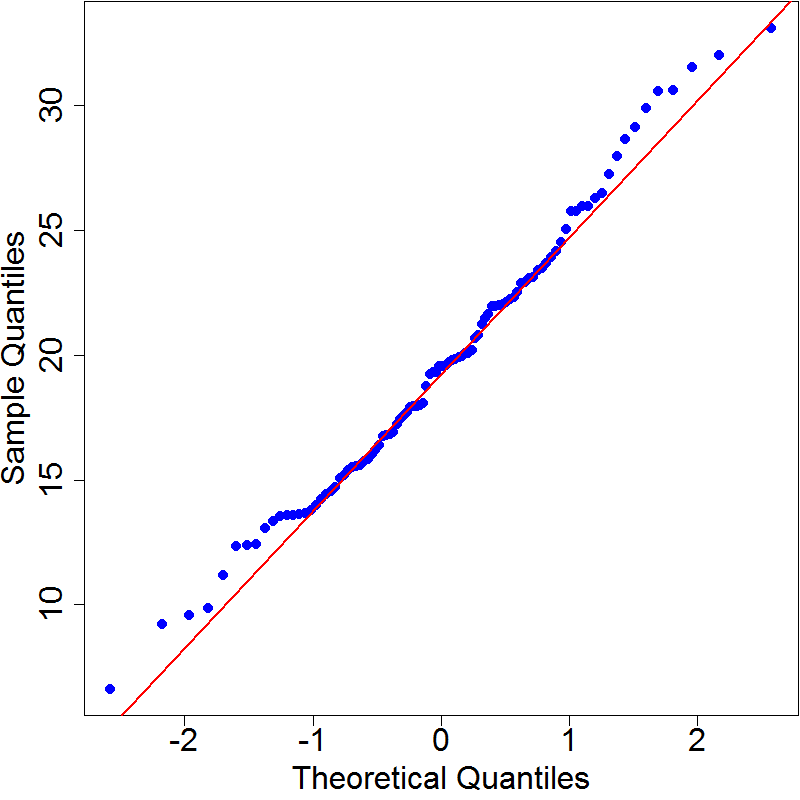
\includegraphics[width=0.5\textwidth]{qqplot.png}
		\end{center}	
	}
	
	\only<2>{
		\begin{center}
			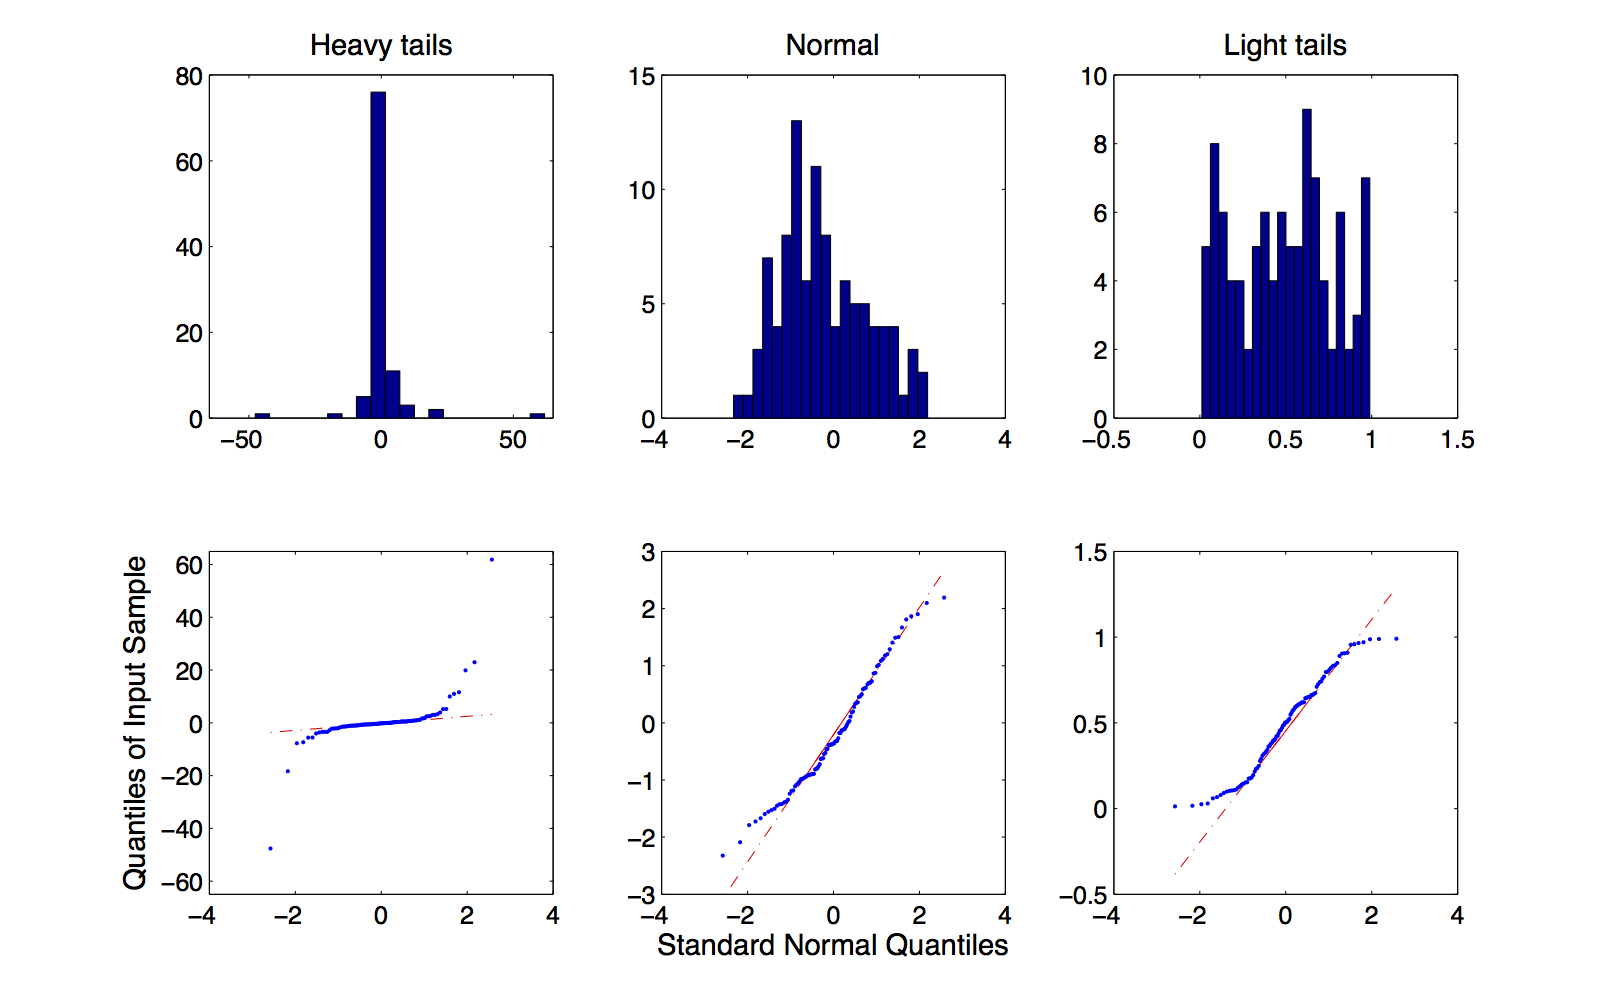
\includegraphics[width=0.9\textwidth,trim=20mm 5mm 20mm 5mm,clip]{qq_tails.png}
		\end{center}		
	}
	
	\only<3>{
		\begin{center}
			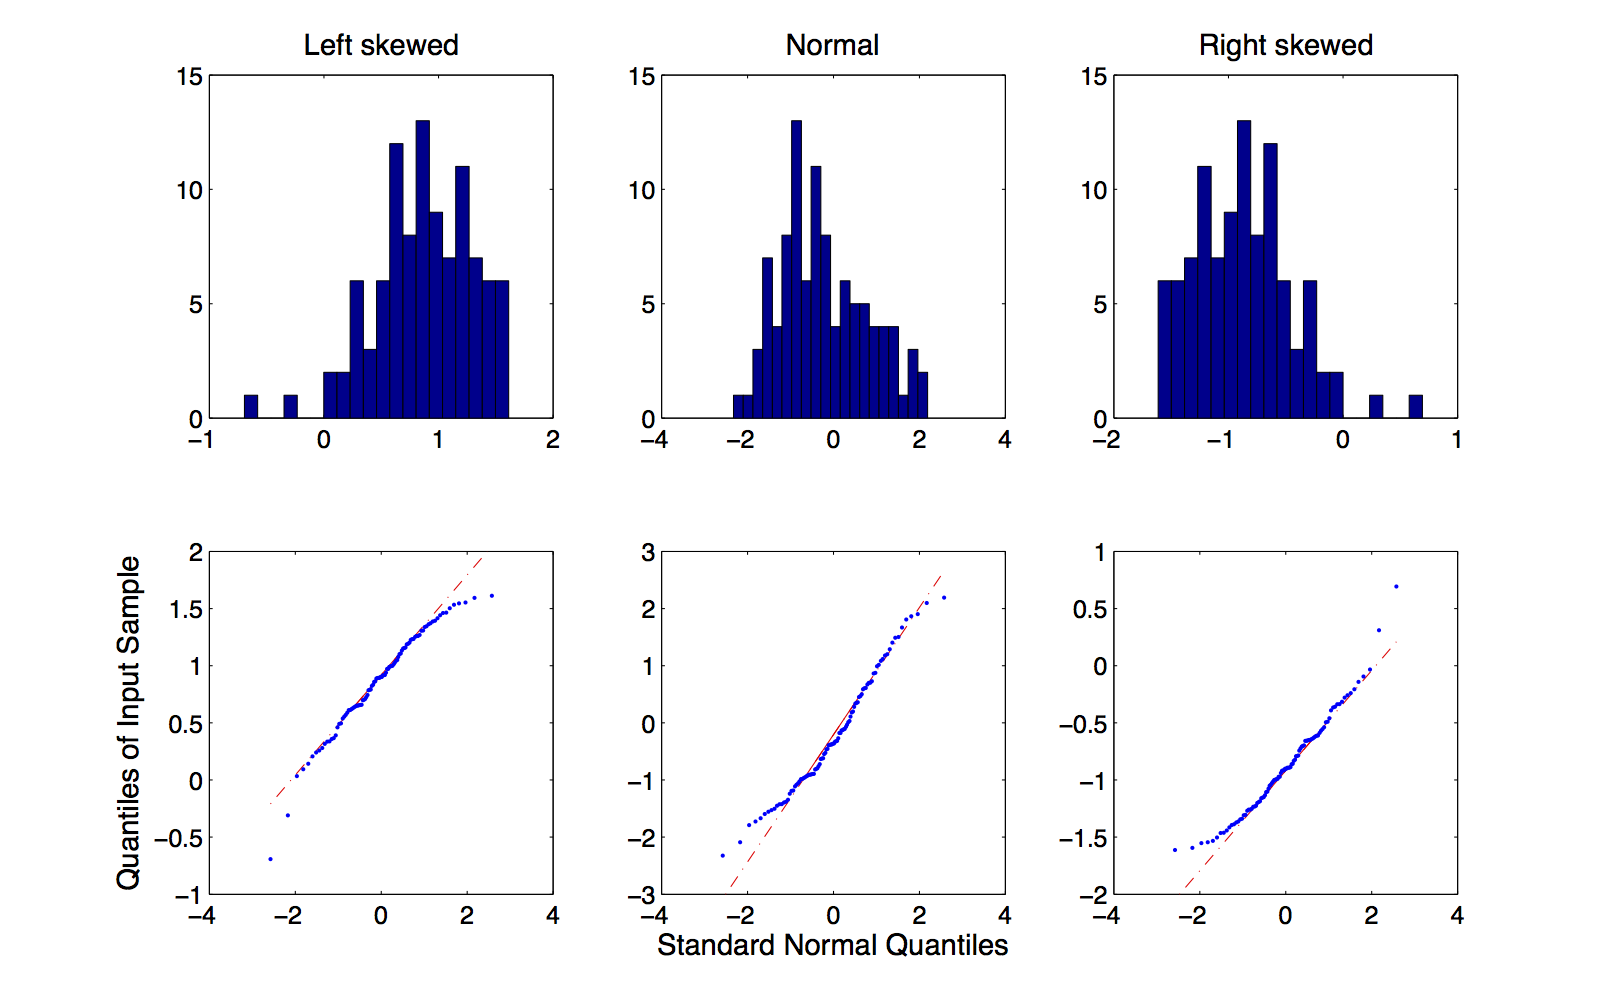
\includegraphics[width=0.9\textwidth,trim=20mm 5mm 20mm 5mm,clip]{qq_skewness.png}
		\end{center}		
	}        
\end{frame}


\begin{frame}{Критерий Шапиро-Уилка}
%%%%%%%%%%%%%%%%%%%%%%%%%%%%%%%%%%%%%%%%%%%%%%%%%%%%%%%%%%%%%%%%%%%%%%%
% Статистика W рассчитывается на основании вариационного ряда, полученного из выборки, и некоторых величин a. Эти величины основаны на математических ожиданиях порядковых статистик из стандартного нормального распределения, они табулированы, для них не существует аналитических выражений. Кроме того, табулировано и нулевое распределение статистики критерия Шапиро-Уилка, то есть его невозможно записать аналитически. Используя таблицы этих величин, можно вычислить достигаемый уровень значимости.
%%%%%%%%%%%%%%%%%%%%%%%%%%%%%%%%%%%%%%%%%%%%%%%%%%%%%%%%%%%%%%%%%%%%%%%
	\begin{center}
		\begin{tabular}{rl}
			выборка:                        & $X^n=\left(X_1,\ldots,X_n\right)$         \\
			нулевая гипотеза:               & $H_0\colon X \sim N\left(\mu,\sigma^2\right)$ \\
			альтернатива:                   & $H_1\colon H_0$ неверна \\
			статистика:                     & $W \left(X^n\right) = \frac{\left(\sum\limits_{i=1}^n a_i X_{(i)}\right)^2}{\sum\limits_{i=1}^n\left(X_i-\bar{X}\right)^2}$ \\
			& $\left(a_1,\ldots,a_n\right) = \frac{m^TV^{-1}}{\left(m^TV^{-1}V^{-1}m\right)^{1/2}}$ \\
			& $m=\left(m_1,\ldots,m_n\right)^T$ --- матожидания порядковых \\
			& статистик $N(0,1)$, $V$ --- их ковариационная матрица \\
			нулевое распределение:          & табличное\\
		\end{tabular}
	\end{center}
	Значения $a_i$ также табулированы.
\end{frame}

\begin{frame}{Итого о проверке нормальности}
	\only<1>{
%%%%%%%%%%%%%%%%%%%%%%%%%%%%%%%%%%%%%%%%%%%%%%%%%%%%%%%%%%%%%%%%%%%%%%%
% Какой из рассмотренных критериев лучше использовать?
%%%%%%%%%%%%%%%%%%%%%%%%%%%%%%%%%%%%%%%%%%%%%%%%%%%%%%%%%%%%%%%%%%%%%%%
		\begin{itemize}
            \large
			\item \textbf{выбросы}: сильно влияют на выборочные коэффициенты асимметрии и эксцесса
            \bigskip
			\item \textbf{критерий Лиллиефорса}: представляет только исторический интерес
            \bigskip
			\item \textbf{критерий хи-квадрат}: слишком общий, не самый мощный, потеря информации из-за разбиения на интервалы
		\end{itemize}
	}
	\only<2>{
%%%%%%%%%%%%%%%%%%%%%%%%%%%%%%%%%%%%%%%%%%%%%%%%%%%%%%%%%%%%%%%%%%%%%%%
% В справочнике Кобзаря показано, что критерий Шапиро-Уилка обладает достаточно хорошей мощностью для разных классов альтернатив.
%%%%%%%%%%%%%%%%%%%%%%%%%%%%%%%%%%%%%%%%%%%%%%%%%%%%%%%%%%%%%%%%%%%%%%%
		\begin{center}
			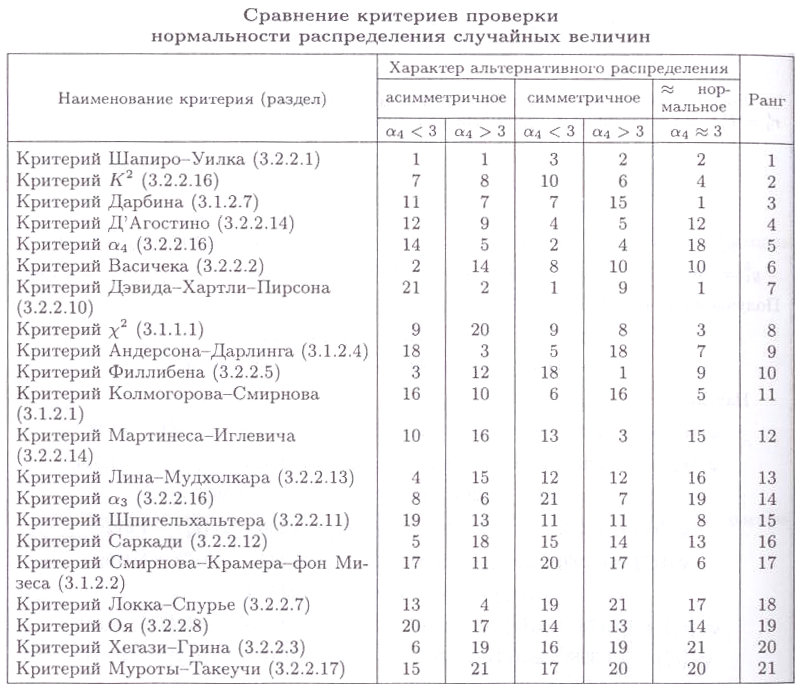
\includegraphics[height=0.8\textheight]{kobzar.png}
		\end{center}
		Кобзарь, 3.2.2.19, табл.~80.
	}
	
	\only<3>{
%%%%%%%%%%%%%%%%%%%%%%%%%%%%%%%%%%%%%%%%%%%%%%%%%%%%%%%%%%%%%%%%%%%%%%%
% Давайте сделаем шаг назад и подумаем, зачем нужно формально проверять нормальность.
% Дело в том, что проверка гипотезы нормальности наследует плохие свойства всего аппарата проверки гипотез: на маленьких выборках нулевая гипотеза, как правило, не отклоняется, а на выборках огромного размера — практически наверняка отклоняется. То есть, если выборка маленькая, то, формально проверяя гипотезу о нормальности, ее? не получается отклонить, а если выборка огромна, то гипотеза отклоняется, даже если распределение отличается от нормального совсем чуть-чуть.
% Многие методы, предполагающие нормальность, в том числе критерии Стьюдента, нечувствительны к небольшим отклонениям от нормальности, то есть истинное распределение выборки может слегка отличаться от нормального, и t-критерий будет все? еще правильно работать. Нормальное распределение — это математический конструкт. Никаких нормальных выборок в природе не существует. Однако, как говорил Джордж Бокс: «Все модели неверны, а некоторые полезны» — а нормальные модели очень полезны, поэтому их имеет смысл использовать.
%%%%%%%%%%%%%%%%%%%%%%%%%%%%%%%%%%%%%%%%%%%%%%%%%%%%%%%%%%%%%%%%%%%%%%%
	\large
\begin{itemize}
        
		\item \textbf{очень маленькие выборки}: любой критерий может пропустить отклонения от нормальности, графические методы бесполезны
    \bigskip		
\item \textbf{очень большие выборки}: любой критерий может выявлять небольшие статистически, но не практически значимые отклонения от нормальности; значительная часть методов, предполагающих нормальность, демонстрируют устойчивость к отклонениям от неё
\end{itemize}}
	
	\only<4>{
%%%%%%%%%%%%%%%%%%%%%%%%%%%%%%%%%%%%%%%%%%%%%%%%%%%%%%%%%%%%%%%%%%%%%%%
% В итоге предлагается использовать следующий алгоритм. Если анализируемые данные имеют распределение, явно отличающееся от нормального (например, измеряемый признак — бинарный или категориальный), не нужно применять метод, предполагающий нормальность. Лучше использовать метод, специально разработанный для такого распределения. Если исследуемый признак, по крайней мере, измерен в непрерывной шкале, можно построить Q-Q график. Если на этом графике не видно существенных отклонений от нормальности (точки лежат примерно на прямой), можно использовать методы, устойчивые к небольшим отклонениям от нормальности, например, критерии Стьюдента. Если используемый метод чувствителен к отклонениям от нормальности, необходимо формально проверить нормальность, и рекомендуется это делать с помощью метода Шапиро-Уилка.  Если критерий Шапиро-Уилка отвергает нормальность, не нужно использовать методы, чувствительные к отклонениям от нормальности.
%%%%%%%%%%%%%%%%%%%%%%%%%%%%%%%%%%%%%%%%%%%%%%%%%%%%%%%%%%%%%%%%%%%%%%%
        \large
		\begin{itemize}
			\item если  \textit{данные явно ненормальны} (например, бинарны или дискретны), нужно выбрать метод, специфичный для такого распределения
            \bigskip			
            \item если \textit{на ку-ку графике не видно существенных отклонений от~нормальности}, можно сразу использовать методы, устойчивые к~небольшим отклонениям (например, критерии Стьюдента)
            \bigskip
			\item если метод  \textit{чувствителен к отклонениям от~нормальности} (например, критерий Фишера), проверять её рекомендуется критерием Шапиро-Уилка
            \bigskip
			\item если  \textit{нормальность отвергается}, чувствительные методы, предполагающие нормальность, использовать нельзя!
		\end{itemize}	
	}
\end{frame}


\section{Правдоподобие}
\subsection{Критерии на основе правдоподобия}
\begin{frame}{Критерии на основе правдоподобия}	
	$$X^{n} = \left( X_{1}, \ldots, X_{n} \right), \; X \sim f\left(x, \theta\right).$$
	
	ОМП для $\theta$:
	\begin{align*}
	\log L\left(X^n,\theta\right) &= \sum\limits_{i=1}^n \log f\left(X_i, \theta\right), \\
	\hat{\theta}_{MLE}&= \argmax{\theta} \log L\left( X^n, \theta \right), \\
	I\left(\theta\right) &=   - \frac{\partial^2}{\partial\theta^2}\log L\left(\theta\right), \\
	\mathbb D\hat{\theta}_{MLE} &= I^{-1}\left(\hat{\theta}_{MLE}\right), \\
	S\left(\theta\right) &= \frac{\partial}{\partial \theta} \log L\left( \theta\right).
	\end{align*}
	
	$\hat{\theta}_{MLE}$ и $S\left(\hat{\theta}_{MLE}\right)$ асимптотически нормально распределены.
\end{frame}

\begin{frame}{Критерий Вальда}
	\begin{center}
		\begin{tabular}{rl}
			выборка:                        & $X^n=\left(X_1,\ldots,X_n\right), X\sim F\left(x, \theta\right)$\\
			нулевая гипотеза:               & $H_0\colon \theta=\theta_0$ \\
			альтернатива:                   & $H_1\colon \theta<\neq>\theta_0$ \\
			статистика:                     & $Z_W\left(X^n\right) = \frac{\hat{\theta}_{MLE} - \theta_0}{\sqrt{\mathbb D \hat{\theta}_{MLE}}}$ \\
			нулевое распределение:          & $Z_W\left(X^n\right) \sim N\left(0,1\right)$ при $H_0$\\
		\end{tabular}
		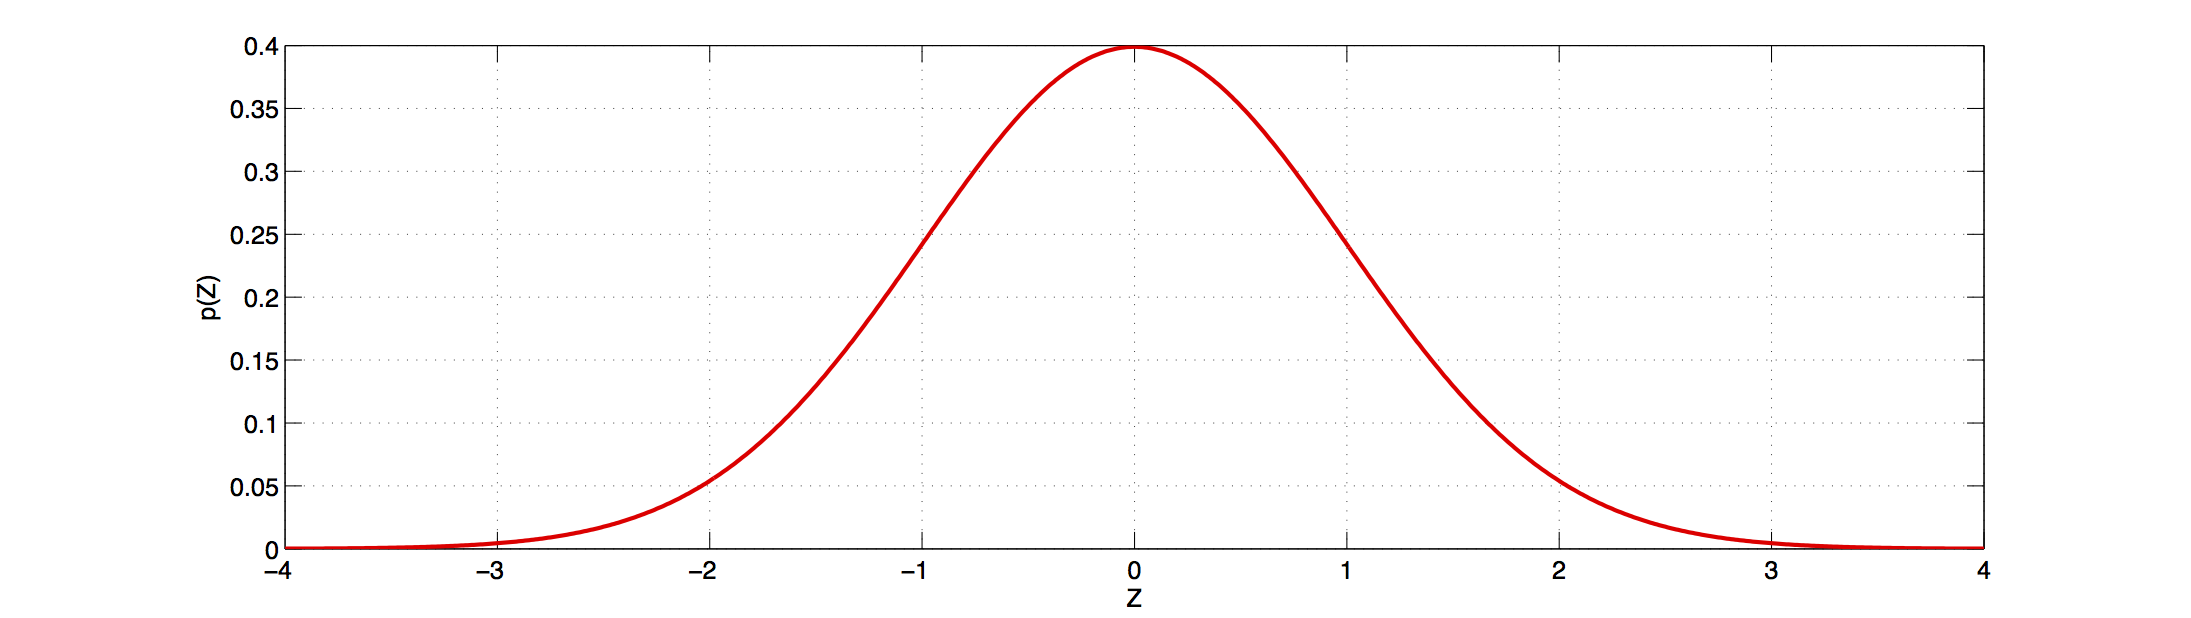
\includegraphics[width=0.7\textwidth]{norm.png}
	\end{center}
	достигаемый уровень значимости:
	$$p\left(Z_W\right) = \begin{cases}
	1-F_{N(0,1)}(Z_W), & H_1 \colon \theta>\theta_0, \\
	F_{N(0,1)}(Z_W), & H_1 \colon \theta<\theta_0, \\
	2\left(1-F_{N(0,1)}(|Z_W|)\right), & H_1 \colon \theta\neq\theta_0. \\
	\end{cases}
	$$
\end{frame}

\begin{frame}{Критерий отношения правдоподобия}
	\begin{center}
		\begin{tabular}{rl}
			выборка:                        & $X^n=\left(X_1,\ldots,X_n\right), X\sim F\left(x, \theta\right)$\\
			нулевая гипотеза:               & $H_0\colon \theta=\theta_0$ \\
			альтернатива:                   & $H_1\colon \theta\neq\theta_0$ \\
			статистика:                     & $LR\left(X^n\right) = -2\log \frac{L\left(X^n, \theta_0\right)}{L\left(X^n, \hat{\theta}_{MLE}\right)}$ \\
			нулевое распределение:          & $LR\left(X^n\right) \sim \chi^2_1$ при $H_0$\\
		\end{tabular}
		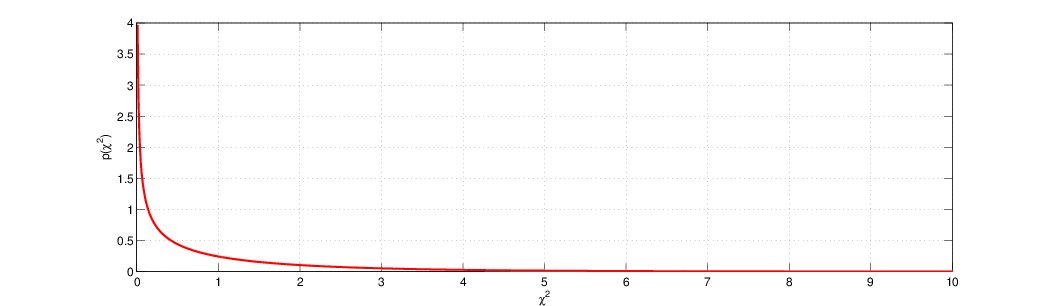
\includegraphics[width=0.7\textwidth]{chi21.png}
	\end{center}
	достигаемый уровень значимости: 
	$$p\left(LR\right) = 1 - F_{\chi^2_1}\left(LR\right).$$
	
	Если $\theta$~--- вектор размерности $k$, то нулевое распределение критерия~--- $\chi^2_k.$
\end{frame}

\begin{frame}{Критерий меток}
	\begin{center}
		\begin{tabular}{rl}
			выборка:                        & $X^n=\left(X_1,\ldots,X_n\right), X\sim F\left(x, \theta\right)$\\
			нулевая гипотеза:               & $H_0\colon \theta=\theta_0$ \\
			альтернатива:                   & $H_1\colon \theta<\neq>\theta_0$ \\
			статистика:                     & $Z_S\left(X^n\right) = \frac{S\left(\theta_0\right)}{\sqrt{I\left(\theta_0\right)}}$ \\
			нулевое распределение:          & $N\left(0,1\right)$\\
		\end{tabular}
		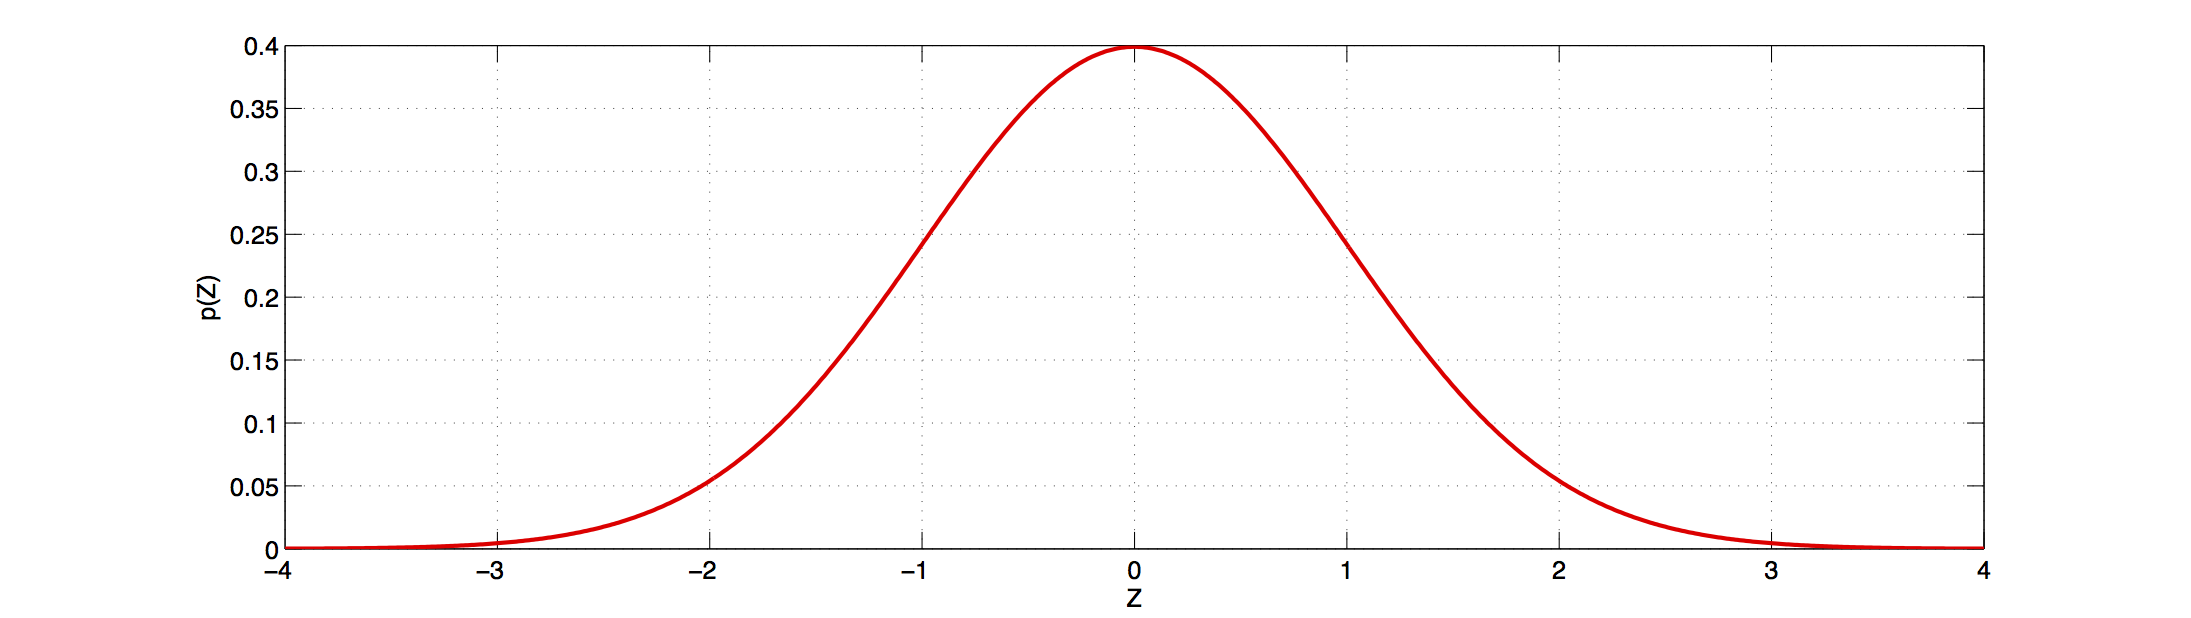
\includegraphics[width=0.7\textwidth]{norm.png}
	\end{center}
	достигаемый уровень значимости:
	$$p\left(Z_S\right) = \begin{cases}
	1-F_{N(0,1)}(Z_S), & H_1 \colon \theta>\theta_0, \\
	F_{N(0,1)}(Z_S), & H_1 \colon \theta<\theta_0, \\
	2\left(1-F_{N(0,1)}(|Z_S|)\right), & H_1 \colon \theta\neq\theta_0. \\
	\end{cases}
	$$
\end{frame}

\begin{frame}{Три критерия}
	\begin{figure}
		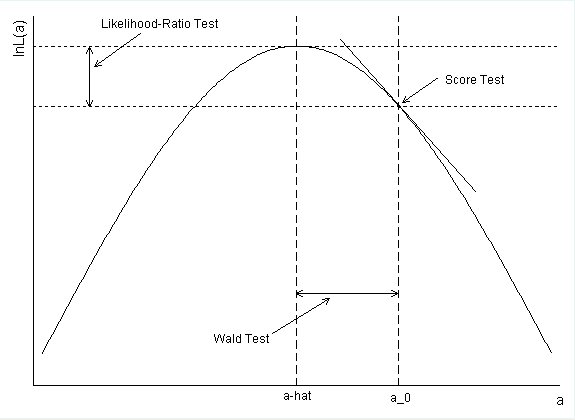
\includegraphics[width=0.5\textwidth]{nested_tests.png}
	\end{figure} 
	\begin{itemize}
		\item критерий Вальда использует информацию о~правдоподобии только в~$\hat{\theta}_{MLE}$, критерий меток~--- только в $\theta_0$, критерий отношения правдоподобия~--- в обеих точках
		\item все три критерия асимптотические; на конечных выборках хуже всего критерий Вальда
	\end{itemize}

\end{frame}

\section{Распределение Бернулли}
%%%%%%%%%%%%%%%%%%%%%%%%%%%%%%%%%%%%%%%%%%%%%%%%%%%%%%%%%%%%%%%%%%%%%%%
% Еще? одно семейство параметрических критериев — это критерии, которые работают с распределениями Бернулли. Они принимают на вход выборки из нулей и единиц и проверяют гипотезы о параметрах p этих распределений (вероятность появления единицы в выборке). С распределением Бернулли работать удобно потому, что, в отличие от нормального распределения, не нужно применять никаких методов, чтобы доказать, что выборка взята именно из этого распределения. Если случайная величина принимает только 2 значения, то она имеет распределение Бернулли.
% Далее будут рассмотрены критерии, решающие три задачи: одновыборочную, двухвыборочную с независимыми выборками и двухвыборочную со связанными выборками.
%%%%%%%%%%%%%%%%%%%%%%%%%%%%%%%%%%%%%%%%%%%%%%%%%%%%%%%%%%%%%%%%%%%%%%%
\begin{frame}{Распределение Бернулли}	
\only<1>{
	$$X^{n} = \left( X_{1}, \ldots, X_{n} \right), \; X \sim Ber\left(p\right), \; T =\sum\limits_{i=1}^n X_i.$$
	
	ОМП для $p$:
	\begin{align*}
		 L\left(p\right)   &= p^T \left(1-p\right)^{\left(n-T\right)}, \\
		\log L\left(p\right) &= T \ln p + \left(n-T\right) \ln\left(1-p\right), \\
		\hat{p}              &= \frac{T}{n}, \\
		I\left(p\right)      &= -  \frac{\partial^2 \log L(p)}{\partial p^2} = \frac{n}{p\left(1-p\right)}, \\
		\mathbb{D}\hat{p} &= \frac{\hat{p}\left(1-\hat{p}\right)}{n}, \\
		S\left(p\right) &= \frac{T}{p} - \frac{n-T}{1-p}
	\end{align*}
}
\only<2>{
	\begin{align*}
		LR  &= -2\log \frac{L\left(p_0\right)}{L\left(\hat{p}\right)}\sim \chi^2_1 \\
		Z_W &= \frac{\hat{p}-p_0}{\sqrt{1/I\left(\hat{p}\right)}} = \frac{\hat{p}-p_0}{\sqrt{\frac{\hat{p}\left(1-\hat{p}\right)}{n}}} \sim N\left(0,1\right) \\
		Z_S &= \frac{S\left(p_0\right) }{\sqrt{I\left(p_0\right)}} = \frac{\hat{p}-p_0}{\sqrt{\frac{p_0\left(1-p_0\right)}{n}}} \sim N\left(0,1\right)
	\end{align*}
}
\end{frame}

\subsection{Гипотеза о значении одного параметра}
\begin{frame}{Z-критерий меток для доли}
    \only<1>{
    \begin{center}
        \begin{tabular}{rl}
            выборка:                        & $X^{n}=\left(X_{1},\ldots,X_{n}\right), X \sim Ber\left(p\right)$ \\
            нулевая гипотеза:               & $H_0\colon p=p_0$ \\
            альтернатива:                   & $H_1\colon p<\neq>p_0$ \\
            статистика:                     & $Z_S\left(X^{n}\right) = \frac{\hat{p}-p_0}{\sqrt{\frac{p_0\left(1-p_0\right)}{n}}} $ \\
            нулевое распределение:          & $N(0,1)$\\
        \end{tabular}
        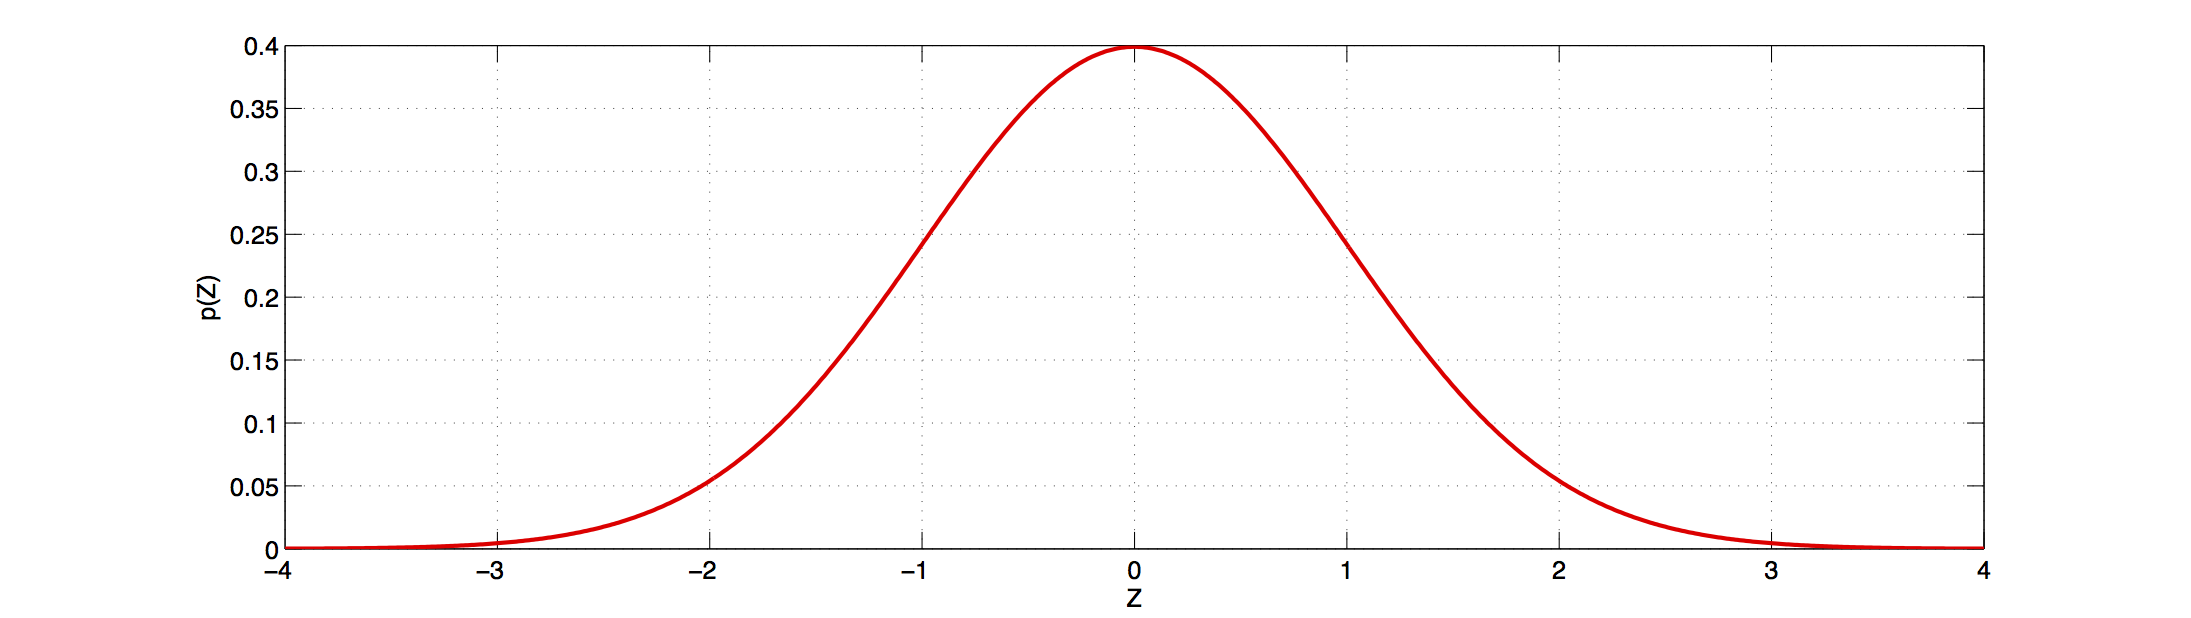
\includegraphics[width=0.7\textwidth]{norm.png}
    \end{center}
    }
\end{frame}

\begin{frame}{Биномиальный критерий}
	\begin{center}
		\begin{tabular}{rl}
			выборка:                        & $X^{n}=\left(X_{1},\ldots,X_{n}\right), X \sim Ber\left(p\right)$ \\
			нулевая гипотеза:               & $H_0\colon p=p_0$ \\
			альтернатива:                   & $H_1\colon p<\neq>p_0$ \\
			статистика:                     & $T\left(X^{n}\right) = \sum\limits_{i=1}^n X_i$ \\
			нулевое распределение:          & $Bin(n,p_0)$\\
		\end{tabular}
		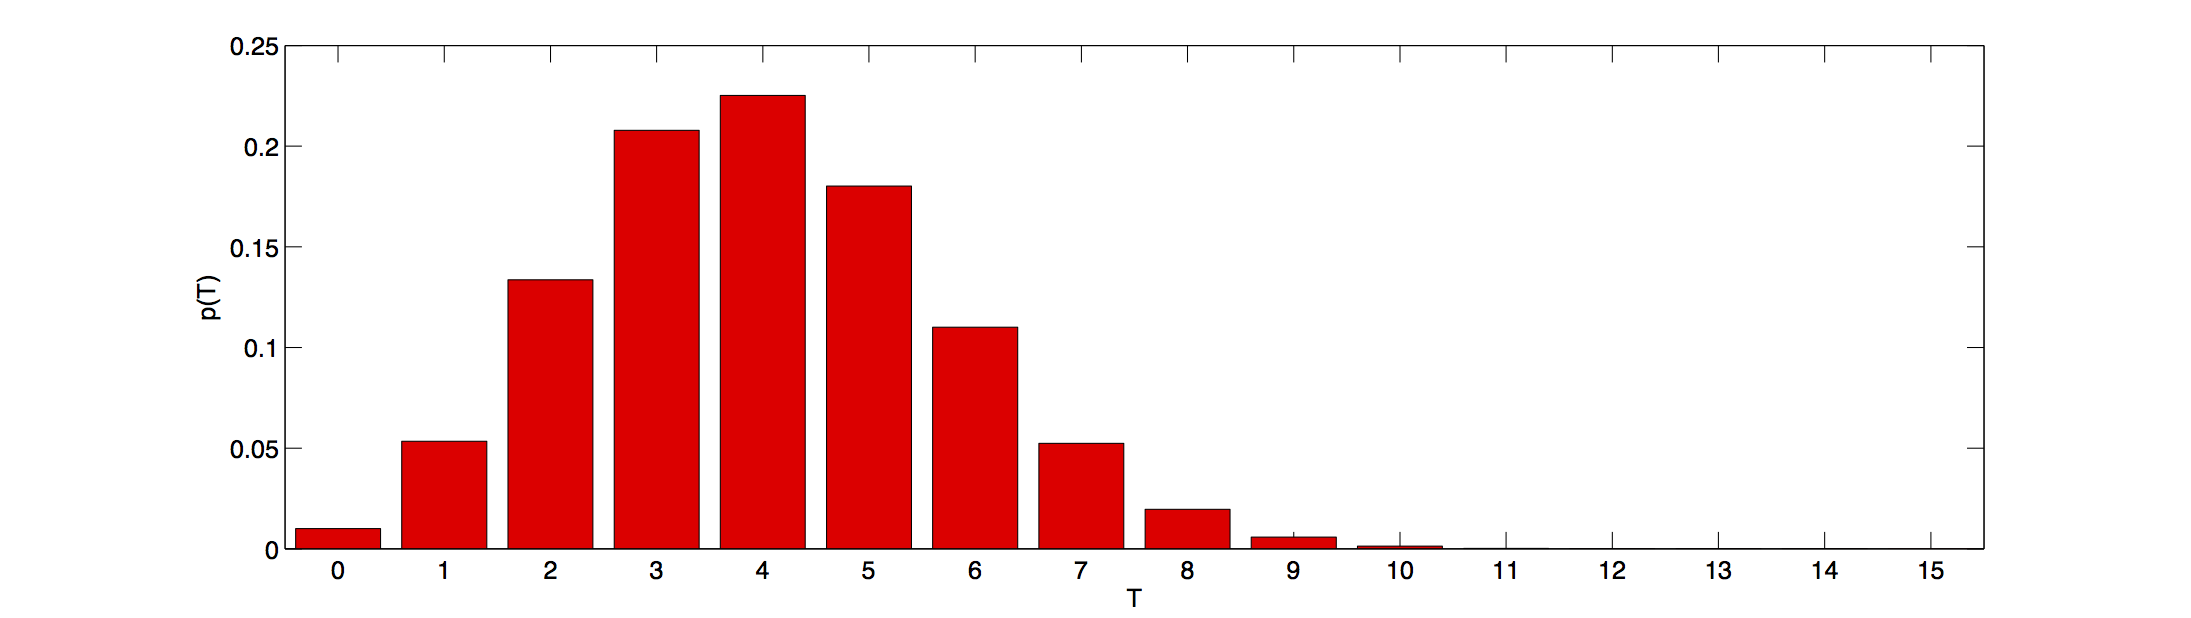
\includegraphics[width=0.7\textwidth]{bin_nonsym.png}
	\end{center}
	
	\vspace{-5pt}
	
	достигаемый уровень значимости:
	$$p\left(T\right) = \begin{cases}
	1-F_{Bin(n,p_0)}(T), & H_1 \colon p>p_0, \\
	F_{Bin(n,p_0)}(T),   & H_1 \colon p<p_0, \\
	\text{через бета-распределение},       & H_1 \colon p\neq p_0. \\
	\end{cases}
	$$
	
	\vspace{-5pt}
	
	Поскольку нулевое распределение дискретно, нельзя добиться, чтобы вероятность ошибки первого рода была равна в точности~$\alpha$. 
\end{frame}

\begin{frame}{Примеры}
\only<1>{
    \begin{block}{Королёв, задача 7.2.2}
    Бенджамин Спок, знаменитый педиатр и автор большого количества книг по воспитанию детей, был арестован за участие в антивоенной демонстрации в Бостоне.
    Его дело должен был рассматривать суд присяжных.
    Присяжные назначаются с помощью многоступенчатой процедуры, на очередном этапе которой было отобрано 300~человек.
    Однако среди них оказалось только 90~женщин.
    Адвокаты доктора Спока подали протест на предвзятость отбора.
    \end{block}
    \bigskip
    
    $H_0\colon$ процедура отбора была беспристрастной, женщины попадали в~выборку с вероятностью $1/2$.
    
    $H_1\colon$ предпочтение отдавалось кандидатам-мужчинам.	
    
    \bigskip
    
    \begin{center}
    	\begin{tabular}{rl}
    		Критерий                & $p$ \\
			Z-критерий меток        & $2.3\times 10^{-12}$ \\
			Z-критерий Вальда       & $2.1\times 10^{-12}$ \\
			Биномиальный            & $1.6\times 10^{-12}$ \\
    	\end{tabular}
    \end{center}    
}

\only<2>{
     \begin{block}{Кобзарь, задача 227} 
    Нормируемый уровень дефектных изделий в партии $p_0=0.05.$
    Среди 20 изделий партии проверка обнаружила 2 дефектных.
    \end{block}
    \bigskip
    
    $H_0\colon$ доля дефектных изделий в~партии не выше нормы.
    
    $H_1\colon$ доля дефектных изделий в~партии выше нормы.
    
    \bigskip
        
    \textbf{Обратите внимание}: если $H_0\colon p=p_0$ проверяется против $H_1\colon p>p_0$, ничего не изменится от замены нулевой гипотезы на $H_0\colon p\leq p_0$.
    
    \bigskip
    
    \begin{center}
    	\begin{tabular}{rl}
    		Критерий                & $p$ \\
    		Z-критерий меток        & $0.1524$ \\
    		Z-критерий Вальда       & $0.2280$ \\ 
    		Биномиальный            & $0.2642$ \\
    	\end{tabular}
    \end{center}        	
}
\end{frame}


\begin{frame}{Доверительные интервалы для доли}
    \only<1>{
    Доверительный интервал Вальда основывается на аппроксимации нормальным распределением:  
    $$F_X\left(x\right) \approx \Phi \left(\frac{x-Np}{\sqrt{Np\left(1-p\right)}}\right)$$.

    $100\left(1-\alpha\right)$\% доверительный интервал Вальда:

    \bigskip

    \begin{center}
    	\begin{tabular}{rll}
    		Метод                   & Пример 1           & Пример 2 \\
    		Вальда                  & $[0.2481, 0.3519]$ & $[-0.0315, 0.2315]$\\
    	\end{tabular}
    \end{center}  

	\bigskip
	
    \textbf{Недостатки:}
    \begin{itemize}
    \item доверительные пределы могут выходить за границы $\left[0,1\right]$ (вообще, при $\hat{p}\in\left(0,1\right)$ нежелательно даже $C_L=0$ и $C_U=1$)
    \item при $\hat{p}=0$ и $\hat{p}=1$ вырождается в точку
    \item антиконсервативен~--- накрывает $p$ реже, чем в $100\left(1-\alpha\right)$\% случаев
    \end{itemize}
    }

    \only<2>{
    Более точный доверительный интервал Уилсона (основан на критерии меток):
    $$\frac{\hat{p}+z_{1-\frac{\alpha}{2}}/2}{n+z_{1-\frac{\alpha}{2}}} \pm \frac{z_{1-\frac{\alpha}{2}}\sqrt{n}}{n+z_{1-\frac{\alpha}{2}}^2}  \sqrt{\hat{p}\left(1-\hat{p}\right) + \frac{z_{1-\frac{\alpha}{2}}^2}{4n}}$$

    \bigskip

    \begin{center}
    	\begin{tabular}{rll}
    		Метод                   & Пример 1           & Пример 2 \\
    		Вальда                  & $[0.2481, 0.3519]$ & $[-0.0315, 0.2315]$\\
    		Уилсона                 & $[0.2509, 0.3541]$ & $[0.0279, 0.3010]$ \\
    	\end{tabular}
    \end{center}  
}
    \only<3>{
    Доверительный интервал Клоппера-Пирсона (основан на биномиальном критерии) определяется квантилями бета-распределения.

    \bigskip

    \begin{center}
    	\begin{tabular}{rll}
    		Метод                   & Пример 1 & Пример 2 \\
    		Вальда                  & $[0.2481, 0.3519]$ & $[-0.0315, 0.2315]$\\
    		Уилсона                 & $[0.2509, 0.3541]$ & $[0.0279, 0.3010]$ \\
    		Клоппера-Пирсона        & $[0.2486, 0.3553]$ & $[0.0123, 0.3170]$\\      
    	\end{tabular}
    \end{center}     
    
 
 \bigskip
 
 Особенности:
 \begin{itemize}
 	\item всегда точен~--- уровень доверия никогда не ниже номинального
 	\item почти всегда консервативен~--- уровень доверия часто выше номинального
 \end{itemize}    
}
    
    \only<4>{
    Эксперименты при $n=40$:
    \begin{center}
    	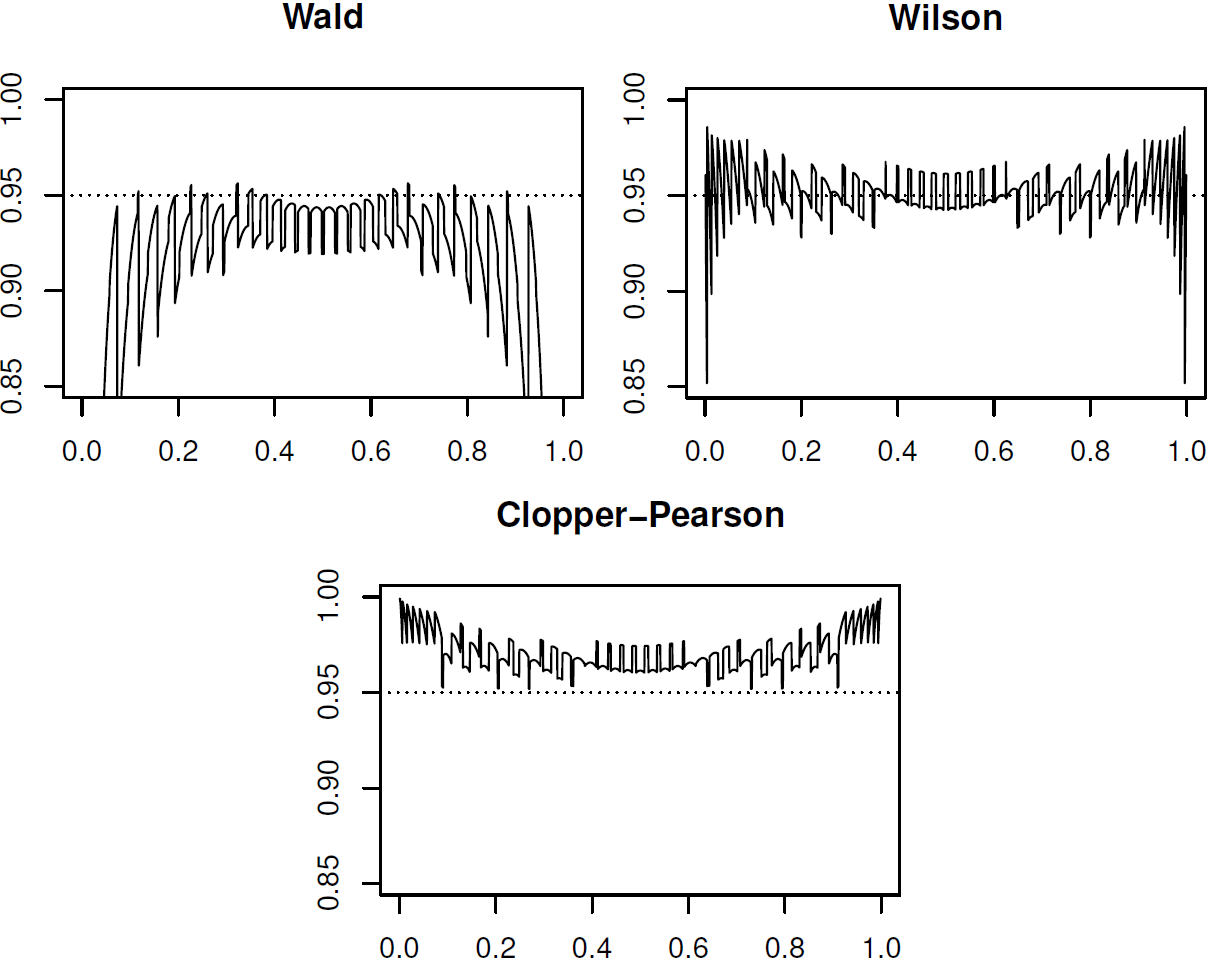
\includegraphics[height=0.8\textheight]{CIs_square.png}
    \end{center}        
    }    
\end{frame}

\subsection{Гипотеза о значениях двух параметров, независимые выборки}
\begin{frame}{Z-критерий для разности двух долей, независимые выборки}
    \only<1>{
%%%%%%%%%%%%%%%%%%%%%%%%%%%%%%%%%%%%%%%%%%%%%%%%%%%%%%%%%%%%%%%%%%%%%%%
%  Когда выборки независимы, то из четыре?х чисел a, b, c, d в таблице сопряже?нности Z-критерий использует только два, стоящие в первой строчке (количество единиц в первой и во второй выборках)
%%%%%%%%%%%%%%%%%%%%%%%%%%%%%%%%%%%%%%%%%%%%%%%%%%%%%%%%%%%%%%%%%%%%%%%
    \small
    \begin{center}
        \begin{tabular}{rl}
            выборки:                        & $X_1^{n_1}=\left(X_{11},\ldots,X_{1n_1}\right), X_{1} \sim Ber\left(p_1\right)$ \\
                                            & $X_2^{n_2}=\left(X_{21},\ldots,X_{2n_2}\right), X_{2} \sim Ber\left(p_2\right)$ \\
                                            & выборки независимы

                                   \vspace{3pt}

                                                \\
            \multicolumn{2}{c}{     \begin{tabular}{|c|c|c|}
                                        \hline
                                        \diagbox{Исход}{Выборка} & $X_1^{n_1}$ & $X_2^{n_2}$ \\\hline
                                        1                            & $a$         & $b$\\\hline
                                        0                            & $c$         & $d$ \\\hline
                                        $\sum$                       & $n_1$       & $n_2$\\\hline
                                    \end{tabular}
                               } \\

                                   \vspace{3pt}
                               
            нулевая гипотеза:               & $H_0\colon p_1=p_2$ \\
            альтернатива:                   & $H_1\colon p_1<\neq>p_2$ \\
            статистика:                     & $Z\left(X_1^{n_1}, X_2^{n_2}\right) = \frac{\hat{p}_1-\hat{p}_2}{\sqrt{P\left(1-P\right)\left(\frac1{n_1}+\frac1{n_2}\right)}}$ \\
            & $P = \frac{\hat{p}_1 n_1 + \hat{p}_2 n_2}{n_1+n_2}, \; \hat{p}_1 = \frac{a}{n_1}, \;\hat{p}_2 = \frac{b}{n_2}$ \\
            нулевое распределение:          & $N(0,1)$\\
        \end{tabular}
        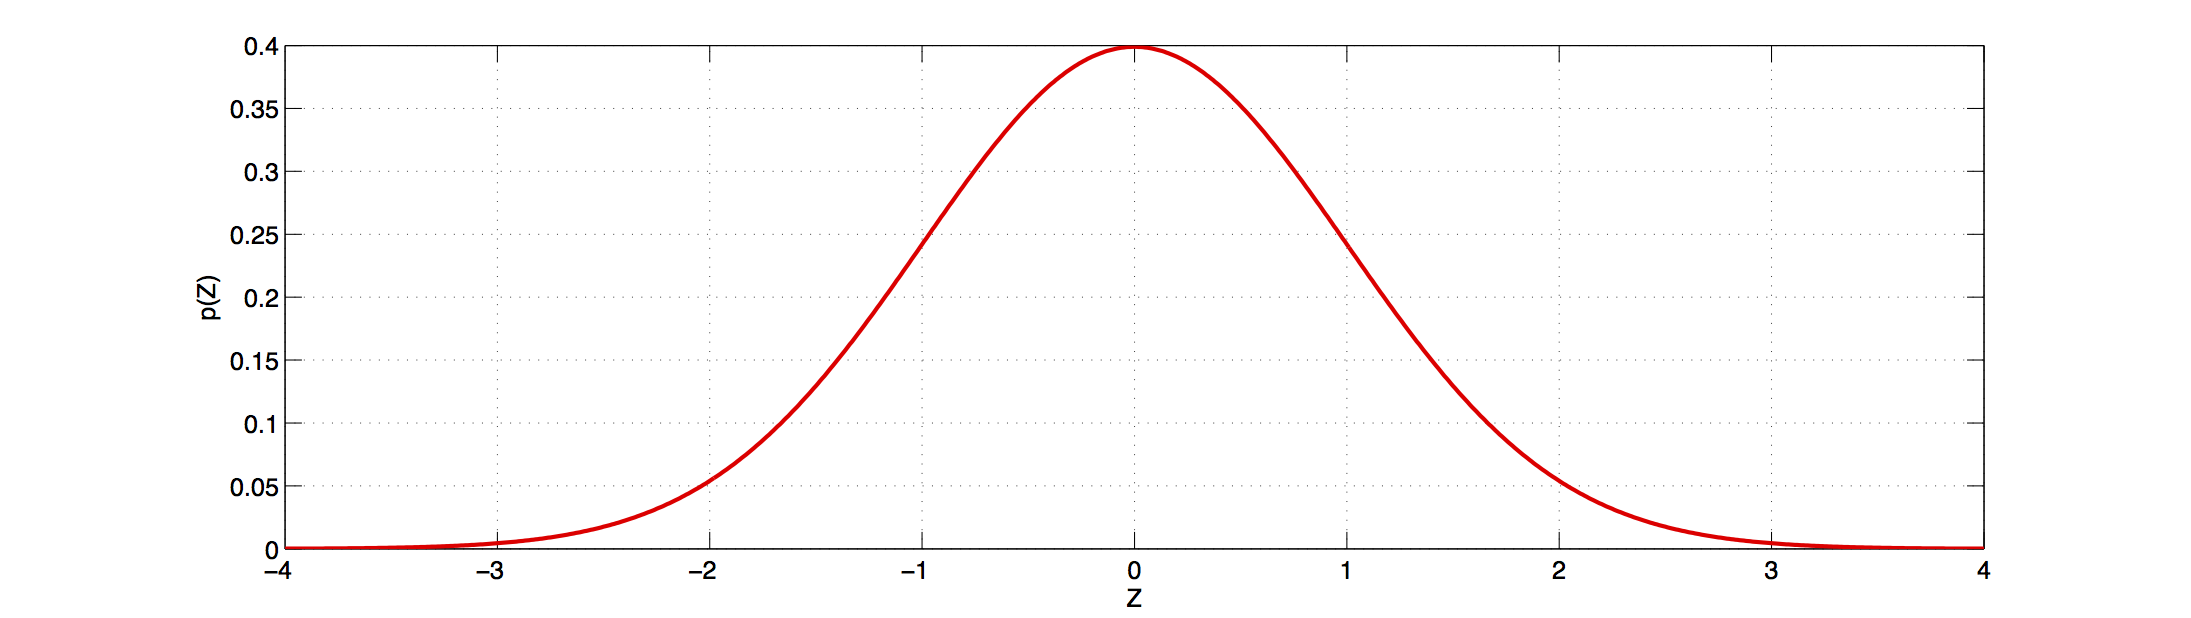
\includegraphics[width=0.7\textwidth]{norm.png}
    \end{center}
    }

    \only<2>{
    \begin{block}{Кобзарь, задача 226}
    В~двух партиях объёмами $n_1=100$~шт. и~$n_2=200$~шт. обнаружено соответственно $t_1=3$ и $t_2=5$ дефектных приборов.
    Необходимо проверить гипотезу о равенстве долей дефектных приборов в~партиях.
    \end{block}
    \bigskip

    \begin{center}
    \begin{tabular}{|c|c|c|}
        \hline
        \diagbox{Наличие дефекта}{Номер партии}&1        &2\\\hline
        Есть                                        &$a=3$    &$b=5$\\\hline
        Нет                                         &$c=97$   &$d=195$ \\\hline
        Всего                                       &$n_1=100$& $n_2=200$\\\hline
    \end{tabular}
    \end{center}

    \bigskip

    $H_0\colon$ доли дефектных изделий в~партиях равны.

    $H_1\colon$ доли дефектных изделий в~партиях различаются $\Rightarrow p = 0.8$.

    $H_1\colon$ доля дефектных изделий в~первой партии выше $\Rightarrow p = 0.4$.

    $H_1\colon$ доля дефектных изделий в~первой партии ниже $\Rightarrow p = 0.6$.
    }
\end{frame}

\begin{frame}{Доверительный интервал для разности двух долей}
    Доверительный интервал Уилсона:
    \begin{align*}
        \left[C_L, C_U\right] &= \left[\hat{p}_1-\hat{p}_2 - \delta, \hat{p}_1-\hat{p}_2 + \varepsilon\right], \\
        \delta                &= z_{1-\frac{\alpha}{2}} \sqrt{\frac{l_1\left(1-l_1\right)}{n_1} + \frac{u_2\left(1-u_2\right)}{n_2}}, \\
        \varepsilon           &= z_{1-\frac{\alpha}{2}} \sqrt{\frac{u_1\left(1-u_1\right)}{n_1} + \frac{l_2\left(1-l_2\right)}{n_2}}, \\
    \end{align*}

    \vspace{-5pt}

    $l_1, u_1$~--- корни уравнения $\left|x-\hat{p}_1\right| = z_{1-\frac{\alpha}{2}} \sqrt{\frac{x\left(1-x\right)}{n_1}}$,

    $l_2, u_2$~--- корни уравнения $\left|x-\hat{p}_2\right| = z_{1-\frac{\alpha}{2}} \sqrt{\frac{x\left(1-x\right)}{n_2}}$.

    \bigskip

    В примере 95\% доверительный интервал~--- $[-0.0331, 0.0616],$ минимальное значение~$\alpha$, при котором интервал не содержит нуля~---  $0.8003$.
\end{frame}

\subsection{Гипотеза о значениях двух параметров, связанные выборки}
\begin{frame}{Z-критерий для разности двух долей, связанные выборки}
    \only<1>{
%%%%%%%%%%%%%%%%%%%%%%%%%%%%%%%%%%%%%%%%%%%%%%%%%%%%%%%%%%%%%%%%%%%%%%%
%  В Z-критерии для связанных выборок используется статистика, в которую входят только внедиагональные элементы f, g таблицы 2 ? 2, то есть только те объекты, на которых значения двух признаков отличаются. Объекты e и h, на которых значения признаков совпадают, в критерии не используются.
%%%%%%%%%%%%%%%%%%%%%%%%%%%%%%%%%%%%%%%%%%%%%%%%%%%%%%%%%%%%%%%%%%%%%%%
    \small
    \begin{center}
        \begin{tabular}{rl}
            выборки:                        & $X_1^n=\left(X_{11},\ldots,X_{1n}\right), X_{1} \sim Ber\left(p_1\right)$ \\
                                            & $X_2^n=\left(X_{21},\ldots,X_{2n}\right), X_{2} \sim Ber\left(p_2\right)$ \\
                                            & выборки связанные

                                   \vspace{3pt}

                                                \\
            \multicolumn{2}{c}{     \begin{tabular}{|c|c|c|}
                                        \hline
                                        \diagbox{$X_1^n$}{$X_2^n$}& 1     & 0    \\\hline
                                        1                              & $e$   & $f$  \\\hline
                                        0                              & $g$   & $h$  \\\hline
                                    \end{tabular}

                                    \vspace{3pt}

                               } \\
                                                \\
            нулевая гипотеза:               & $H_0\colon p_1=p_2$ \\
            альтернатива:                   & $H_1\colon p_1<\neq>p_2$ \\
            статистика:                     & $Z\left(X_1^n, X_2^n\right) = \frac{\hat{p}_1-\hat{p}_2}{\sqrt{\frac{f+g}{n^2}-\frac{\left(f-g\right)^2}{n^3}}} = \frac{f-g}{\sqrt{f+g-\frac{\left(f-g\right)^2}{n}}}$ \\
            нулевое распределение:          & $N(0,1)$\\
        \end{tabular}
        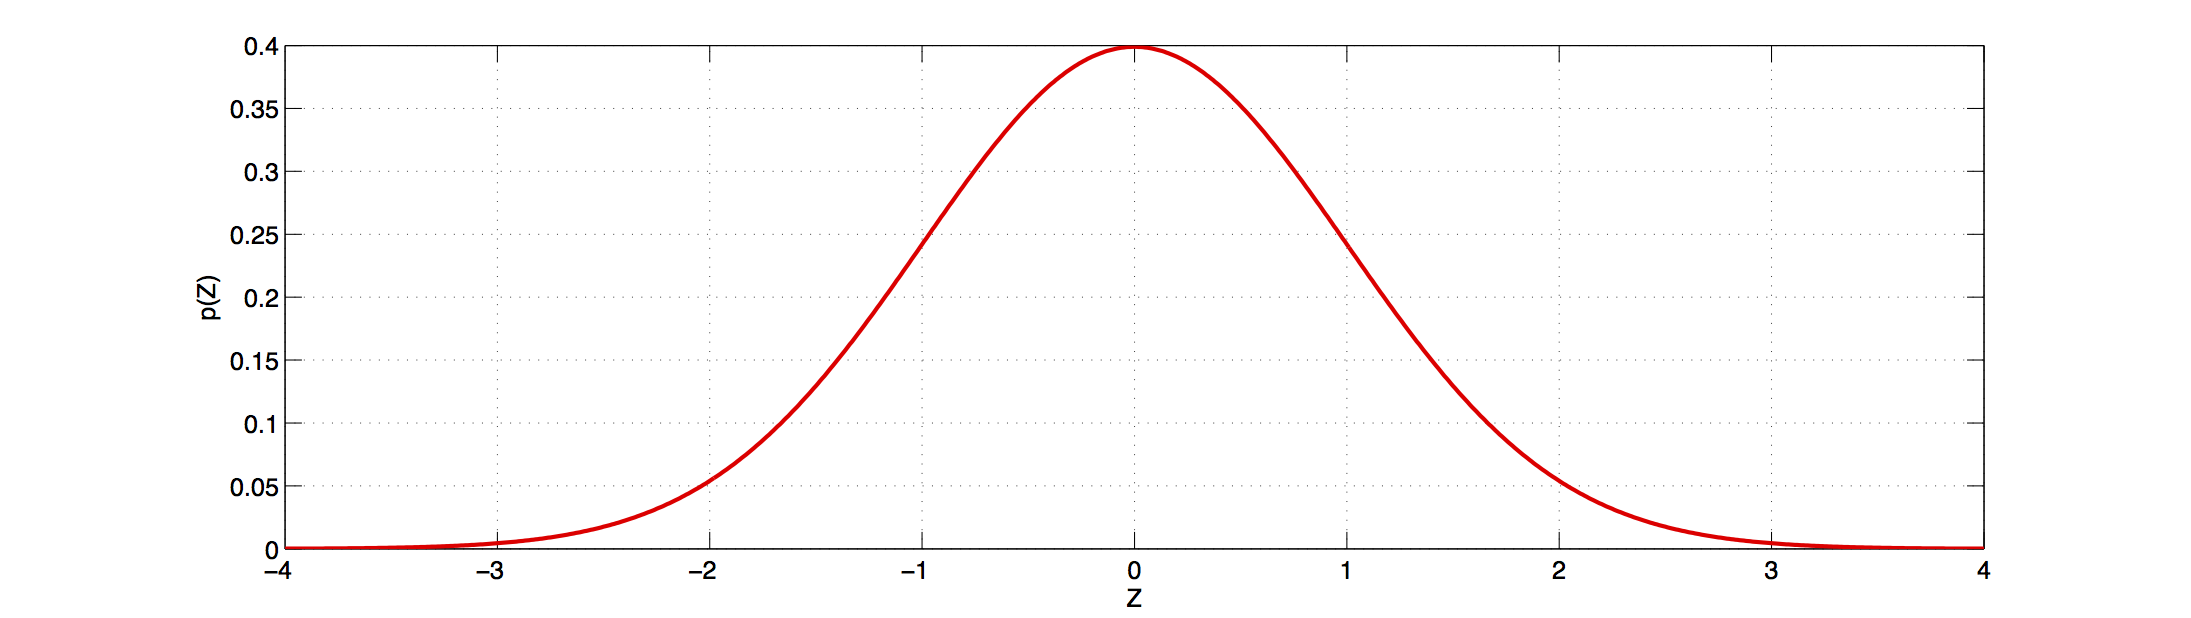
\includegraphics[width=0.7\textwidth]{norm.png}
    \end{center}
    }

    \only<2>{
    \begin{block}{Пример, Agresti, табл.~10.1} Из~опрошенных 1600~граждан Великобритании, имеющих право голоса, 944 высказали одобрение деятельности премьер-министра. 
    Через 6~месяцев эти же люди были опрошены снова, на этот раз одобрение высказали только 880~опрошенных.
    \end{block}
    \bigskip

    \begin{center}
    \begin{tabular}{|c|c|c|c|}
        \hline
        \diagbox{I}{II} & +      & -       & $\sum$\\\hline
        +                    &$e=794$ & $f=150$ & $944$ \\\hline
        -                    &$g=86$  & $h=570$ & $656$ \\\hline
        $\sum$               &$880$   & $720$   & $1600$\\\hline
    \end{tabular}
    \end{center}

    \bigskip

    $H_0\colon$ рейтинг премьер-министра не изменился.

    $H_1\colon$ рейтинг премьер-министра изменился $\Rightarrow p = 2.8\times10^{-5}$.

    $H_1\colon$ рейтинг премьер-министра снизился  $\Rightarrow p = 1.4\times10^{-5}$.

    $H_1\colon$ рейтинг премьер-министра повысился $\Rightarrow p = 0.99999$.
    }

    \only<3>{
    Без учёта информации о связи между выборками:

    \bigskip

    \begin{center}
    \begin{tabular}{|c|c|c|}
        \hline
        \diagbox{Результат}{Опрос} & I          & II      \\\hline
        +                               &$a=944$     & $b=880$ \\\hline
        -                               &$c=656$     & $d=720$ \\\hline
        $\sum$                          &$n_1=1600$  & $n_2=1600$  \\\hline
    \end{tabular}
    \end{center}

    \bigskip

    $H_0\colon$ рейтинг премьер-министра не изменился.

    $H_1\colon$ рейтинг премьер-министра изменился $\Rightarrow p = 0.0222$.

    $H_1\colon$ рейтинг премьер-министра снизился  $\Rightarrow p = 0.0112$.

    $H_1\colon$ рейтинг премьер-министра повысился $\Rightarrow p = 0.9889$.
    }
\end{frame}

\begin{frame}{Доверительный интервал для разности двух долей}
    Доверительный интервал Уилсона:
    \begin{align*}
        \left[C_L, C_U\right] &= \left[\hat{p}_1-\hat{p}_2 - \delta, \hat{p}_1-\hat{p}_2 + \varepsilon\right], \\
        \delta                &= \sqrt{dl_1^2 - 2\hat{\phi}dl_1 du_2 + du_2^2}, \\
        \varepsilon           &= \sqrt{du_1^2 - 2\hat{\phi}du_1 dl_2 + dl_2^2}, \\
        \hat{\phi}             &= \begin{cases}
                                    \frac{eh-fg}{\left(e+f\right)\left(g+h\right)\left(e+h\right)\left(f+h\right)}, & \text{ если знаменатель не равен нулю}, \\
                                    0, & \text{ иначе};
                                 \end{cases}   \\
        dl_1                  &= \hat{p}_1 - l_1, \\
        du_1                  &= u_1 - \hat{p}_1, \\
        dl_2                  &= \hat{p}_2 - l_2, \\
        du_2                  &= u_2 - \hat{p}_2, \\
    \end{align*}

    \vspace{-15pt}

    $l_1, u_1$~--- корни уравнения $\left|x-\hat{p}_1\right| = z_{1-\frac{\alpha}{2}} \sqrt{\frac{x\left(1-x\right)}{n}}$,

    $l_2, u_2$~--- корни уравнения $\left|x-\hat{p}_2\right| = z_{1-\frac{\alpha}{2}} \sqrt{\frac{x\left(1-x\right)}{n}}$.

	\bigskip
	
    В примере 95\% доверительный интервал~--- $[2.14, 5.90]\%,$ минимальное значение~$\alpha$, при котором интервал не содержит нуля~--- $3.1 \times 10^{-5}$.

\end{frame}

\section{}
\begin{frame}{Литература}
    \only<1>{
    Критерии нормальности:
    \begin{itemize}
    \item Харке-Бера (Jarque–Bera)~--- Кобзарь, 3.2.2.16
    \item Шапиро-Уилка (Shapiro-Wilk)~--- Кобзарь, 3.2.2.1
    \item хи-квадрат (chi-square)~--- Кобзарь, 3.1.1.1, 3.2.1.1
    \item согласия (goodness-of-fit), основанные на эмпирической функции распределения ~--- Кобзарь, 3.1.2, 3.2.1.2
    \end{itemize}

	\bigskip

    Для нормальных распределений:
	\begin{itemize}
		\item Z-критерии (Z-tests)~--- Kanji, №№ 1, 2, 3
		\item t-критерии Стьюдента (t-tests)~--- Kanji, №№ 7, 8, 9
		\item критерий хи-квадрат (chi-square test)~--- Kanji, №15
		\item критерий Фишера (F-test)~--- Kanji, №16
	\end{itemize}

	\bigskip

     Критерии, основанные на правдоподобии: Bilder, раздел B.5
    }

    \only<2>{
	Для распределения Бернулли:
	\begin{itemize}
		\item всё про одновыборочную задачу~--- Agresti, 1.3, 1.4
		\item Z-критерии (Z-tests)~--- Kanji, №№ 4, 5
		\item точный критерий (exact binomial test)~--- McDonald, \url{http://www.biostathandbook.com/exactgof.html}
		\item доверительные интервалы Уилсона (score confidence intervals)~--- Newcombe, 1998a, 1998b, 1998c
	\end{itemize}        

    \bigskip

    {\small
     Agresti A. \textit{Categorical Data Analysis}, 2013.
		
    \vspace{5pt}	

    Bilder C.R., Loughin T.M. \textit{Analysis of Categorical Data with R}, 2013.
		
	\vspace{5pt}

	Kanji G.K. \textit{100 statistical tests}, 2006.
	
	\vspace{5pt}	

    McDonald J.H. \textit{Handbook of Biological Statistics}, 2008.
		
	\vspace{5pt}

    Newcombe R.G. (1998). \textit{Two-sided confidence intervals for the single proportion: comparison of seven methods}. Statistics in Medicine, 17, 857–872.		
		
	\vspace{5pt}
	
	Newcombe R.G. (1998). \textit{Interval estimation for the difference between independent proportions: comparison of eleven methods}. Statistics in Medicine, 17, 873–890. 		
		
	\vspace{5pt}
		
	Newcombe R.G. (1998). \textit{Improved confidence intervals for the difference between binomial proportions based on paired data}. Statistics in Medicine, 17, 2635–2650.    		
    
    \vspace{5pt}
    \href{https://stats.idre.ucla.edu/other/mult-pkg/faq/general/faqhow-are-the-likelihood-ratio-wald-and-lagrange-multiplier-score-tests-different-andor-similar/}{О сравнении ассимптотических критериев, ссылка}
    }
    }
    
    \only<3>{{\small
     Кобзарь А.И. \textit{Прикладная математическая статистика}, 2006.       
    
    \vspace{5pt}
    
    Королёв В.Ю. \textit{Теория вероятностей и математическая статистика}, 2008.          
		
	\vspace{5pt}
		    
    NIST/SEMATECH. \textit{e-Handbook of Statistical Methods}. \url{http://www.itl.nist.gov/div898/handbook/}  
	}
    
    }
\end{frame}

\end{document}
